
\begin{appendices}
	\section*{Appendices}
	\begin{enumerate}
		\item Cryptic exon motifs found by \textit{HOMER}\\
		\item All mouse cryptic exons discovered by \textit{CryptEx}\\ 
		\item All human cryptic exons discovered by\textit{CryptEx}\\
		
		\item Calibration of motif enrichment RNA maps using AG and GT dinucleotids
	\end{enumerate}

\clearpage	

%% APPENDICES

\section{Appendices to \autoref{chapter:cryptic_exons} }

\begin{figure}
	\begin{center}
		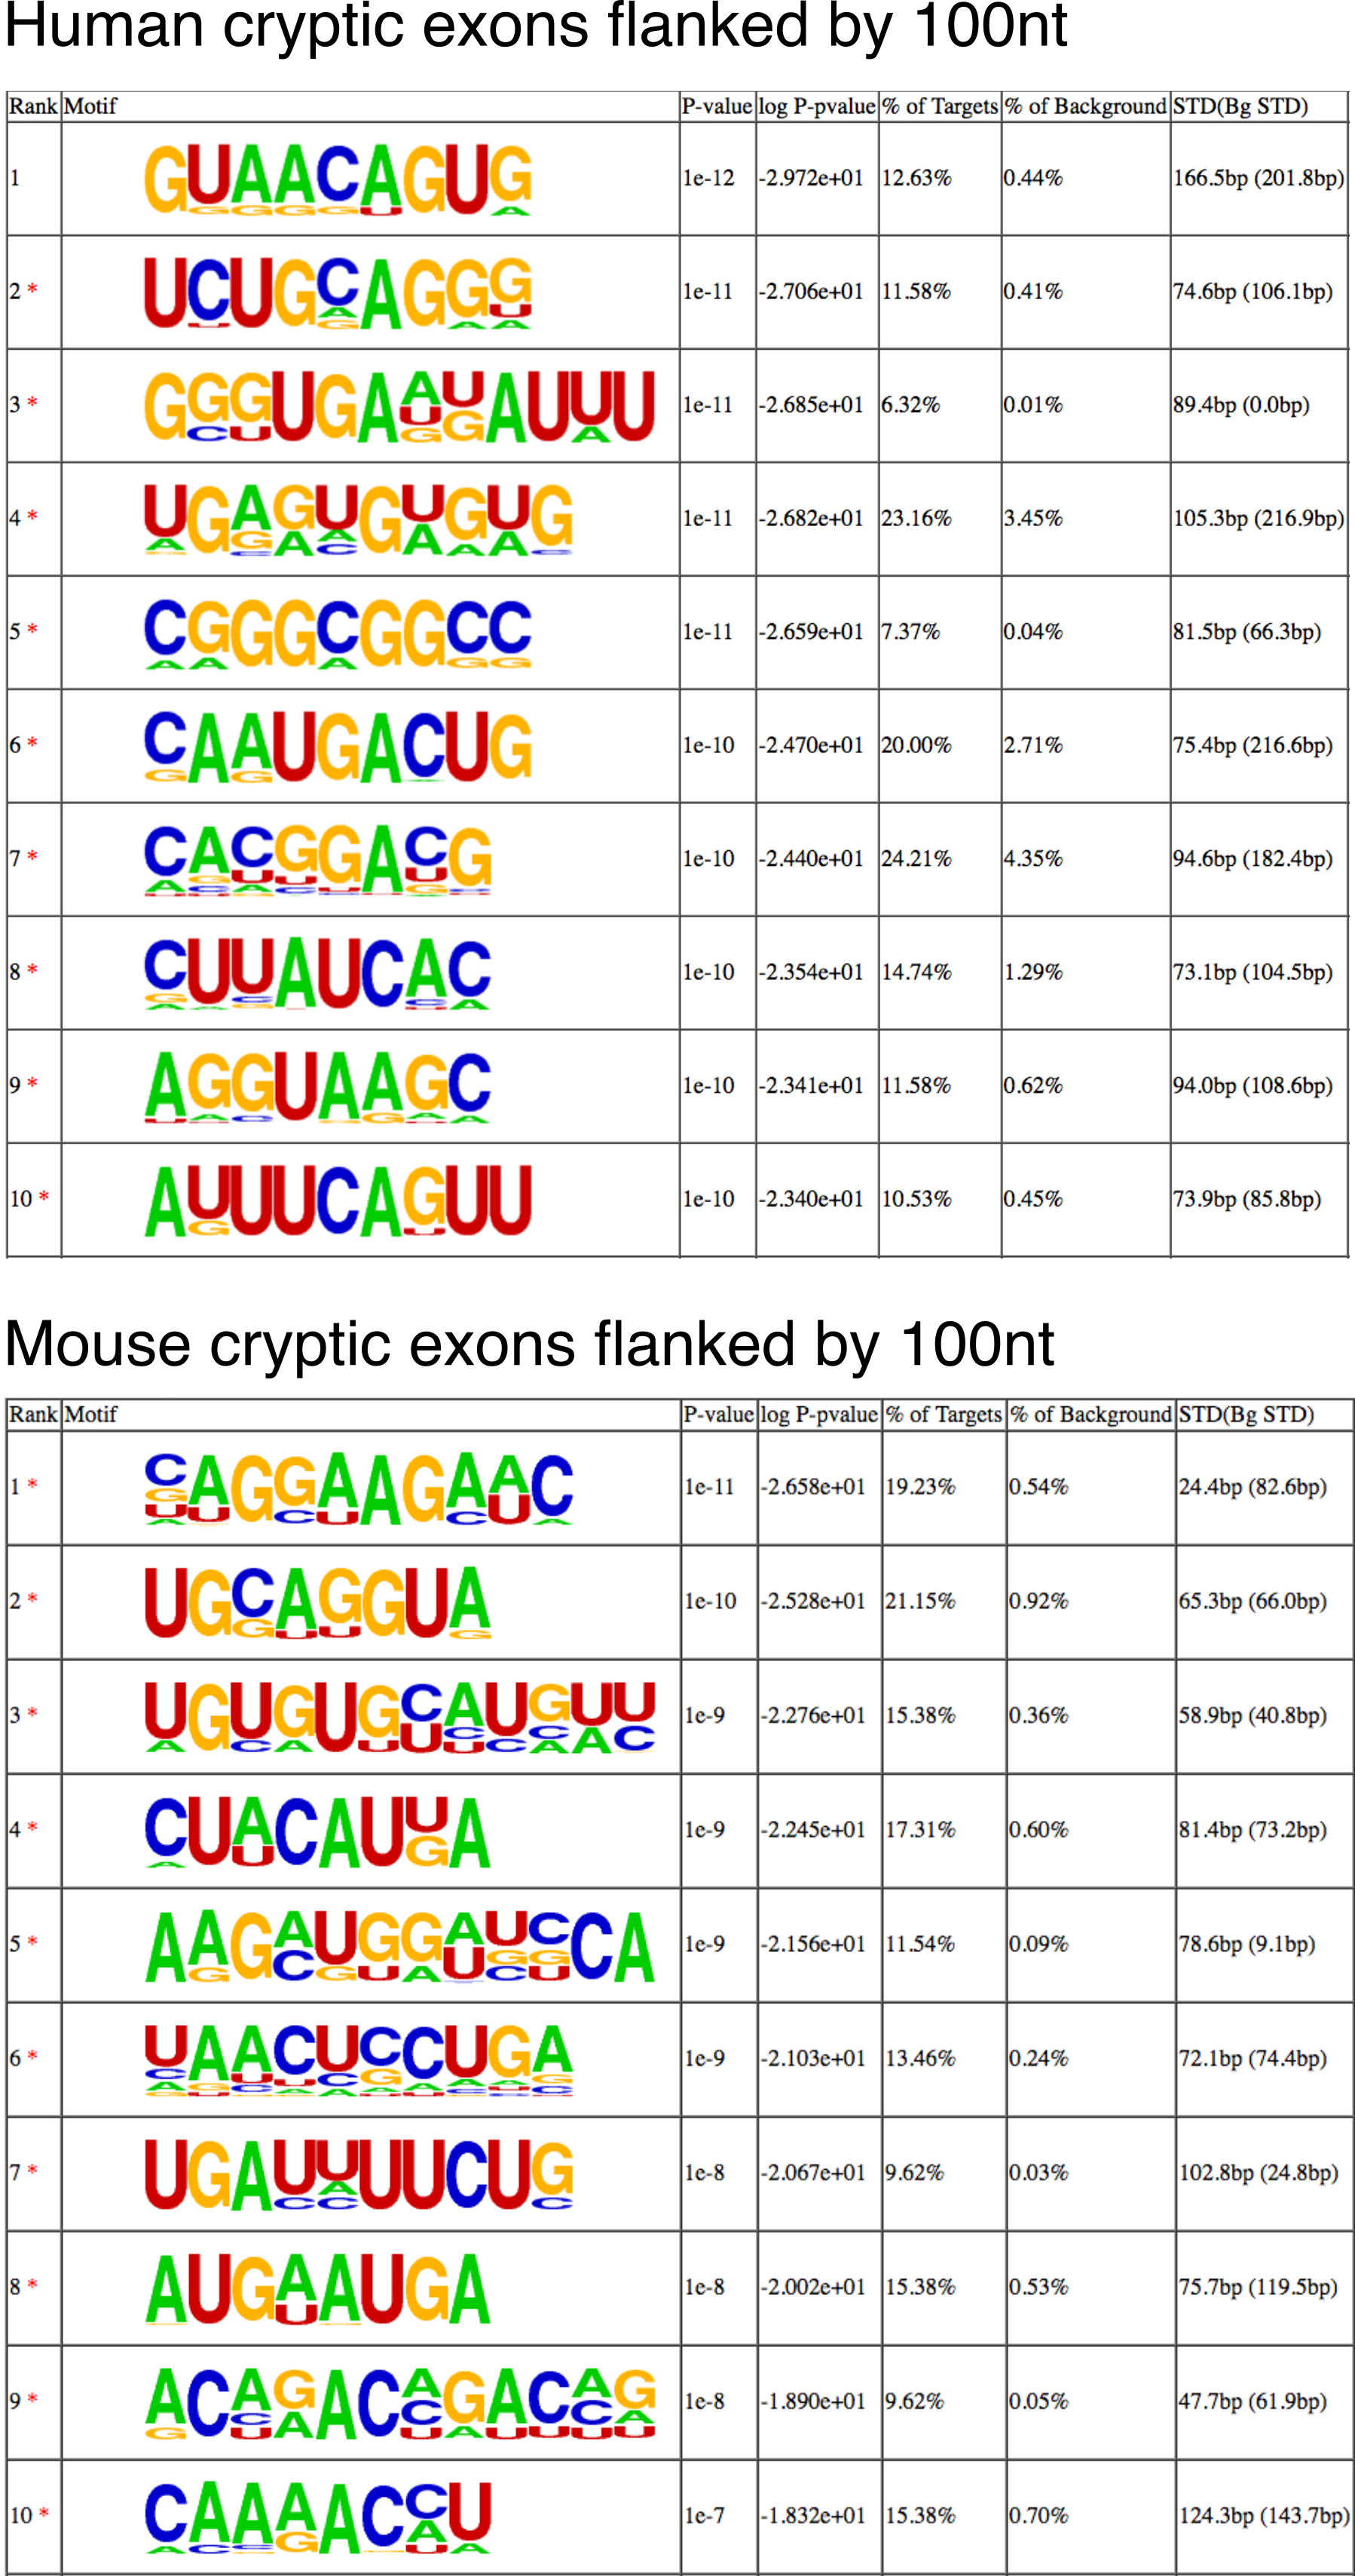
\includegraphics[width=10cm]{Figures/03_cryptic_exons/Figure_S4_HOMER.png}
	\end{center}
	\caption{Motifs found by \textit{HOMER}}
\end{figure}

	\addtolength{\abovecaptionskip}{-25mm}
% mouse table
\newgeometry{left=3cm,bottom=0.8cm}


\begin{landscape}
	%\pagenumbering{gobble}

% Table generated by Excel2LaTeX from sheet 'ST1_mouse_summary_table.tsv'
%\begin{table}[htbp]
% Table generated by Excel2LaTeX from sheet 'ST1_mouse_summary_table.tsv'
\begin{table}[htbp]
	\centering
	2. All mouse cryptic exons discovered by \textit{CryptEx}
	\tiny
	\resizebox{\columnwidth}{!}{
	%\caption{All mouse cryptic exons discovered in chapter 3}
	\begin{tabular}{|l|c|l|l|l|l|c|c|c|l|l|l|l|l|l|}
		\hline
		\multicolumn{15}{|c|}{\cellcolor[HTML]{EFEFEF}{}} \\ \hline
		gene & Ensembl ID & exon ID & chr & exon start & exon end &+/-&5'$\Delta$PSI&3'$\Delta$PSI&classification&observed in&EScell $log_2$FC&brain $log_2$FC&\textit{phyloP}&prediction\\
		\hline
		\textit{Abr} & ENSMUSG00000017631 & E026i1 & chr11 & 76468524 & 76468676 & -     & 0.09  & 0.00  & 5' extension & EScell;brain & -1.75 & -0.59 & 0.77  & PTC/frame shifted \\ \hline
		\textit{Pnpla6} & ENSMUSG00000004565 & E016i1 & chr8  & 3524947 & 3525140 & +     & 0.29  & 0.00  & 5' extension & brain & -1.56 & -0.47 & 0.08  & PTC/frame shifted \\ \hline
		\textit{Lrrc49} & ENSMUSG00000047766 & E017i3 & chr9  & 60637648 & 60637695 & -     & 0.06  & 0.00  & 5' extension & brain & -1.19 & -0.25 & 0.17  & PTC/frame shifted \\ \hline
		\textit{Ccdc149} & ENSMUSG00000045790 & E009i3 & chr5  & 52434250 & 52434424 & -     & 0.16  & 0.00  & 5' extension & brain & .     & -0.28 & 0.06  & PTC/frame conserved \\ \hline
		\textit{Ak5} & ENSMUSG00000039058 & E014i6 & chr3  & 152643869 & 152643915 & -     & 0.16  & 0.00  & 5' extension & brain & .     & -0.53 & 0.17  & PTC/frame shifted \\ \hline
		\textit{Kctd10} & ENSMUSG00000001098 & E017i2 & chr5  & 114376677 & 114376866 & -     & 0.07  & 0.01  & 5' extension & brain & .     & .     & 0.02  & PTC/frame shifted \\ \hline
		\textit{Tmem14a} & ENSMUSG00000025933 & E005i1 & chr1  & 21229121 & 21229173 & +     & 0.37  & 0.00  & 5' extension & brain & -1.02 & -0.60 & -0.08 & PTC/frame conserved \\ \hline
		\textit{Apod} & ENSMUSG00000022548 & E006i1 & chr16 & 31298051 & 31298471 & -     & 0.04  & 0.08  & 3' extension & brain & .     & 0.74  & 0.09  & PTC/frame shifted \\ \hline
		\textit{Erbb2ip} & ENSMUSG00000021709 & E026i1 & chr13 & 103862527 & 103862588 & -     & 0.00  & 0.25  & 3' extension & brain & .     & 0.62  & -0.05 & PTC/frame shifted \\ \hline
		\textit{Trim8} & ENSMUSG00000025034 & E001i2 & chr19 & 46506869 & 46506928 & +     & 0.00  & 0.10  & 3' extension & Ling;brain & .     & .     & -0.23 & PTC/frame shifted \\ \hline
		\textit{Usp15} & ENSMUSG00000099088 & E015i3 & chr10 & 123150961 & 123151125 & -     & 0.00  & 0.32  & 3' extension & Ling;brain & .     & .     & 0.15  & PTC/frame conserved \\ \hline
		\textit{Fam135a} & ENSMUSG00000026153 & E008i1 & chr1  & 24022506 & 24022670 & -     & 0.00  & 0.25  & 3' extension & brain & .     & .     & 0.00  & PTC/frame shifted \\ \hline
		\textit{Rasal1} & ENSMUSG00000029602 & E007i1 & chr5  & 120653508 & 120653879 & +     & 0.03  & 0.16  & 3' extension & brain & .     & .     & -0.23 & PTC/frame conserved \\ \hline
		\textit{Brms1l} & ENSMUSG00000012076 & E008i1 & chr12 & 55864624 & 55865091 & +     & 0.04  & 0.23  & 3' extension & brain & -0.81 & .     & 0.14  & PTC/frame conserved \\ \hline
		\textit{Cacna1b} & ENSMUSG00000004113 & E050i1 & chr2  & 24691959 & 24692366 & -     & 0.00  & 0.39  & 3' extension & brain & .     & -0.58 & 0.21  & PTC/frame shifted \\ \hline
		\textit{Nt5c3b} & ENSMUSG00000017176 & E010i1 & chr11 & 100433637 & 100433684 & -     & 0.00  & 0.07  & 3' extension & brain & -1.15 & -0.50 & 0.12  & PTC/frame conserved \\ \hline
		\textit{Spcs2} & ENSMUSG00000035227 & E004i1 & chr7  & 99856412 & 99856514 & -     & 0.01  & 0.29  & 3' extension & Ling;EScell;brain & .     & 0.34  & 0.40  & PTC/frame shifted \\ \hline
		\textit{Ccdc88a} & ENSMUSG00000032740 & E004i8 & chr11 & 29421354 & 29421401 & +     & 0.00  & 0.27  & 3' extension & brain & -1.63 & .     & -0.04 & PTC/frame conserved \\ \hline
		\textit{Adap1} & ENSMUSG00000056413 & E014i3 & chr5  & 139302108 & 139302166 & -     & 0.00  & 0.36  & 3' extension & brain & .     & -0.47 & 0.08  & PTC/frame shifted \\ \hline
		\textit{Ap3b2} & ENSMUSG00000062444 & E031i2 & chr7  & 81490178 & 81490277 & -     & 0.04  & 0.10  & 3' extension & brain & 0.50  & -0.28 & 0.18  & PTC/frame shifted \\ \hline
		\textit{Fam73a} & ENSMUSG00000054942 & E015i2 & chr3  & 152292556 & 152292657 & -     & 0.02  & 0.09  & 3' extension & Ling;brain & -1.39 & -0.63 & -0.04 & PTC/frame shifted \\ \hline
		\textit{Ptprn2} & ENSMUSG00000056553 & E019i11 & chr12 & 117154249 & 117154298 & +     & 0.00  & 0.13  & 3' extension & brain & .     & -1.01 & 0.24  & PTC/frame shifted \\ \hline
		\textit{Dlg2} & ENSMUSG00000052572 & E004i17 & chr7  & 91543136 & 91543191 & +     & 0.00  & 0.23  & 3' extension & brain & .     & -0.71 & 1.67  & PTC/frame shifted \\ \hline
		\textit{Cd200} & ENSMUSG00000022661 & E003i1 & chr16 & 45389970 & 45390184 & -     & 0.04  & 0.06  & 3' extension & brain & .     & .     & -0.13 & Not in CDS \\ \hline
		\textit{Dock4} & ENSMUSG00000035954 & E049i1 & chr12 & 40835769 & 40835912 & +     & 0.09  & 0.20  & Cassette & brain & .     & -0.68 & 0.53  & PTC/frame shifted \\ \hline
		\textit{C4b} & ENSMUSG00000073418 & E032i1 & chr17 & 34739389 & 34739500 & -     & 0.06  & 0.30  & Cassette & brain & .     & .     & 0.00  & PTC/frame shifted \\ \hline
		\textit{Camk1g} & ENSMUSG00000016179 & E017i2 & chr1  & 193368866 & 193368952 & -     & 0.70  & 0.47  & Cassette & brain & .     & .     & -0.06 & Not in CDS  \\ \hline
		\textit{Reep3} & ENSMUSG00000019873 & E001i1 & chr10 & 67014087 & 67014164 & -     & 0.67  & 0.39  & Cassette & brain & .     & 0.44  & -0.01 & PTC/frame shifted \\ \hline
		\textit{Drosha} & ENSMUSG00000022191 & E009i1 & chr15 & 12833221 & 12833389 & +     & 0.10  & 0.15  & Cassette & brain & .     & .     & -0.06 & PTC/frame conserved \\ \hline
		\textit{Synj2bp} & ENSMUSG00000021139 & E036i2 & chr12 & 81509671 & 81510249 & -     & 0.41  & 0.07  & Cassette & brain & .     & .     & 0.11  & PTC/frame shifted \\ \hline
		\textit{Adnp2} & ENSMUSG00000053950 & E002i1 & chr18 & 80138152 & 80138304 & -     & 0.57  & 0.50  & Cassette & Ling;EScell;brain & 0.33  & 0.25  & 0.03  & PTC/frame shifted \\ \hline
		\textit{Adipor2} & ENSMUSG00000030168 & E010i2 & chr6  & 119369859 & 119369918 & -     & 0.30  & 0.44  & Cassette & Ling;brain & -1.06 & .     & 0.07  & PTC/frame shifted \\ \hline
		\textit{Cdh22} & ENSMUSG00000053166 & E013i2 & chr2  & 165183238 & 165183371 & -     & 0.40  & 0.67  & Cassette & brain & .     & -0.35 & 0.13  & Not in CDS \\ \hline
		\textit{Ermn} & ENSMUSG00000026830 & E001i1 & chr2  & 58049485 & 58049561 & -     & 0.16  & 0.16  & Cassette & brain & .     & .     & 0.06  & PTC/frame shifted \\ \hline
		\textit{Ift81} & ENSMUSG00000029469 & E003i1 & chr5  & 122556905 & 122556991 & -     & 0.19  & 0.08  & Cassette & Ling;brain & .     & .     & 0.08  & benign/frame shifted \\ \hline
		\textit{Vps13d} & ENSMUSG00000020220 & E043i1 & chr4  & 145099351 & 145099463 & -     & 0.60  & 0.20  & Cassette & brain & .     & -0.81 & 0.23  & PTC/frame shifted \\ \hline
		\textit{Ube2d1} & ENSMUSG00000019927 & E010i1 & chr10 & 71263584 & 71263717 & -     & 0.15  & 0.36  & Cassette & EScell;brain & .     & 0.35  & 0.04  & PTC/frame shifted \\ \hline
		\textit{Hgsnat} & ENSMUSG00000037260 & E001i1 & chr8  & 25945947 & 25945999 & -     & 0.28  & 0.15  & Cassette & Ling;brain & -0.59 & .     & 0.20  & PTC/frame conserved \\ \hline
		\textit{Elmod1} & ENSMUSG00000041986 & E003i2 & chr9  & 53923941 & 53923995 & -     & 0.27  & 0.19  & Cassette & brain & .     & .     & 0.97  & benign/frame conserved \\ \hline
		\textit{Mkx} & ENSMUSG00000061013 & E007i7 & chr18 & 6986138 & 6986235 & -     & 0.24  & 0.50  & Cassette & brain & .     & .     & -0.08 & PTC/frame shifted \\ \hline
		\textit{Hace1} & ENSMUSG00000038822 & E013i1 & chr10 & 45639722 & 45639803 & +     & 0.06  & 0.20  & Cassette & Ling;brain & .     & -0.38 & 0.10  & benign/frame conserved \\ \hline
		\textit{Fxyd2} & ENSMUSG00000059412 & E003i1 & chr9  & 45408987 & 45409173 & +     & 0.42  & 0.18  & Cassette & brain & -1.89 & .     & -0.25 & PTC/frame shifted \\ \hline
		\textit{Thoc7} & ENSMUSG00000053453 & E007i1 & chr14 & 13957061 & 13957631 & -     & 0.21  & -0.10 & 5' extension & EScell & -0.74 & .     & 0.04  & PTC/frame shifted \\ \hline
		\textit{Nme6} & ENSMUSG00000032478 & E020i1 & chr9  & 109837872 & 109838225 & +     & 0.40  & 0.00  & 5' extension & Ling;EScell & -0.84 & .     & 0.21  & PTC/frame conserved \\ \hline
		\textit{Wtip} & ENSMUSG00000036459 & E001i1 & chr7  & 34111074 & 34111099 & -     & 0.13  & 0.00  & 5' extension & EScell & -0.46 & .     & 0.26  & PTC/frame shifted \\ \hline
		\textit{Gsta4} & ENSMUSG00000032348 & E005i2 & chr9  & 78207196 & 78207382 & +     & 0.02  & 0.07  & 3' extension & Ling;EScell & -0.45 & .     & 0.11  & PTC/frame shifted \\ \hline
		\textit{Slc7a6} & ENSMUSG00000031904 & E001i1 & chr8  & 106169186 & 106169256 & +     & 0.00  & 0.12  & 3' extension & EScell & .     & -0.23 & -0.25 & Not in CDS \\ \hline
		\textit{Flnb} & ENSMUSG00000025278 & E040i1 & chr14 & 7935368 & 7935630 & +     & 0.09  & 0.43  & Cassette & Ling;EScell;brain & -1.34 & .     & -0.12 & PTC/frame shifted \\ \hline
		\textit{B4galnt3} & ENSMUSG00000041372 & E002i1 & chr6  & 120204263 & 120204465 & -     & 0.07  & 0.10  & Cassette & EScell & .     & .     & -0.15 & PTC/frame shifted \\ \hline
		\textit{Psma2} & ENSMUSG00000015671 & E005i1 & chr13 & 14620930 & 14621038 & +     & 0.06  & 0.13  & Cassette & EScell & .     & .     & 0.19  & PTC/frame conserved \\ \hline
		\textit{Abr} & ENSMUSG00000017631 & E024i1 & chr11 & 76464580 & 76464758 & -     & 0.18  & 0.07  & Cassette & EScell;brain & -1.75 & -0.59 & -0.25 & PTC/frame shifted \\ \hline
		\textit{Wasf3} & ENSMUSG00000029636 & E009i1 & chr5  & 146469766 & 146469912 & +     & 0.10  & 0.22  & Cassette & EScell & .     & .     & -0.02 & benign/frame conserved \\ \hline
	\end{tabular}%
	}
\end{table}%

\clearpage

%% Table generated by Excel2LaTeX from sheet 'ST2_human_summary_table.tsv'
\begin{table}
	\centering
	3. All human cryptic exons discovered by \textit{CryptEx}
	\tiny
	\resizebox{\columnwidth}{!}{ 
%	\fontsize{5}{6}
	\begin{tabular}{|l|c|l|l|l|l|c|c|c|l|l|l|l|l|l|l|l|}
		\hline
%		\multicolumn{17}{Human cryptic exons} \\ 
		\multicolumn{17}{|c|}{\cellcolor[HTML]{EFEFEF}{} } \\ 
		\hline
		gene&Ensembl ID&exon ID&chr&exon start&exon end&+/-& 5'$\Delta$PSI&3'$\Delta$PSI& classification& observed in &mRNA FC&total FC&\textit{phyloP}&prediction&\textit{maxEnt} 5'&\textit{maxEnt} 3'\\ \hline 
		\textit{PHF12} & ENSG00000109118 & E028i1 & chr17 & 28914903 & 28915475 & -     & 0.14  & 0.00  & 5' extension & mRNA;total & 0.23  & . & 0.448493 & PTC/frame conserved & . &  9.93 \\ \hline
		\textit{ZFPM2} & ENSG00000169946 & E016i1 & chr8  & 105419822 & 105419906 & +     & 0.35  & 0.00  & 5' extension & mRNA  & . & . & -0.131815 & PTC/frame conserved & . &  11.28 \\ \hline
		\textit{ACBD3} & ENSG00000182827 & E004i1 & chr1  & 226156701 & 226156780 & -     & 0.12  & 0.00  & 5' extension & mRNA  & -0.31 & . & 0.22671 & PTC/frame shifted & . &  9.63 \\ \hline
		\textit{RPS6KA3} & ENSG00000177189 & E031i2 & chrX  & 20241592 & 20241686 & -     & 0.18  & 0.01  & 5' extension & mRNA  & -0.42 & . & 2.38738 & PTC/frame shifted & . &  8.09 \\ \hline
		\textit{CPED1} & ENSG00000106034 & E034i7 & chr7  & 121194471 & 121194593 & +     & 0.07  & 0.01  & 5' extension & mRNA  & . & . & 0.398074 & PTC/frame shifted & . &  9.56 \\ \hline
		\textit{HUWE1} & ENSG00000086758 & E033i1 & chrX  & 53551990 & 53552074 & -     & 0.09  & 0.05  & 5' extension & mRNA  & -0.56 & . & 0.114241 & PTC/frame shifted & . &  6.87 \\ \hline
		\textit{DYNC2LI1} & ENSG00000138036 & E006i1 & chr2  & 43774402 & 43774936 & +     & 0.08  & 0.04  & 5' extension & mRNA  & -0.63 & . & -0.228969 & PTC/frame shifted & . &  2.09 \\ \hline
		\textit{ZMYND8} & ENSG00000101040 & E019i2 & chr20 & 47254235 & 47254424 & -     & 0.07  & 0.03  & 5' extension & mRNA  & -0.36 & . & 0.101961 & PTC/frame shifted & . &  3.77 \\ \hline
		\textit{HEPH} & ENSG00000089472 & E030i1 & chrX  & 66257344 & 66257516 & +     & 0.12  & 0.00  & 5' extension & mRNA  & -0.58 & -0.34 & 0.245606 & PTC/frame shifted & . &  14.19 \\ \hline
		\textit{BTNL9} & ENSG00000165810 & E031i1 & chr5  & 181059149 & 181059215 & +     & 0.09  & 0.00  & 5' extension & mRNA  & . & . & -0.101275 & PTC/frame shifted & . &  -0.66 \\ \hline
		\textit{PAPSS1} & ENSG00000138801 & E008i1 & chr4  & 107654948 & 107655036 & -     & 0.08  & 0.00  & 5' extension & mRNA;total & -0.87 & . & 0.746813 & PTC/frame conserved & . &  10.84 \\ \hline
		\textit{CLASP1} & ENSG00000074054 & E049i1 & chr2  & 121471187 & 121471274 & -     & 0.16  & 0.00  & 5' extension & mRNA  & -0.19 & . & -0.0460715 & PTC/frame shifted & . &  4.56 \\ \hline
		\textit{IST1} & ENSG00000224470 & E053i1 & chr16 & 71922108 & 71922437 & +     & 0.12  & 0.01  & 5' extension & mRNA  & . & . & 0.177172 & PTC/frame shifted & . &  13.96 \\ \hline
		\textit{UBR4} & ENSG00000272084& E084i1 & chr1  & 19145598 & 19145708 & -     & 0.05  & 0.00  & 5' extension & mRNA  & . & . & 0.710974 & PTC/frame shifted & . &  7.28 \\ \hline
		\textit{ANKRD27} & ENSG00000105186 & E019i1 & chr19 & 32630070 & 32630151 & -     & 0.15  & 0.01  & 5' extension & mRNA  & -0.37 & -0.24 & -0.103821 & PTC/frame shifted & . &  12.52 \\ \hline
		\textit{CCDC77} & ENSG00000120647 & E020i1 & chr12 & 422421 & 422891 & +     & 0.07  & 0.01  & 5' extension & mRNA  & -0.84 & . & -0.0231545 & PTC/frame shifted & . &  3.79 \\ \hline
		\textit{LRPPRC} & ENSG00000138095 & E024i1 & chr2  & 43942675 & 43942815 & -     & 0.06  & 0.00  & 5' extension & mRNA  & -1.01 & . & 0.14133 & PTC/frame shifted & . &  3.85 \\ \hline
		\textit{ADGRV1} & ENSG00000164199 & E085i1 & chr5  & 90803514 & 90803596 & +     & 0.07  & 0.00  & 5' extension & mRNA  & -0.47 & 0.32  & -0.185377 & PTC/frame shifted & . &  9.14 \\ \hline
		\textit{ASNSP1} & ENSG00000248498 & E006i1 & chr8  & 46595259 & 46595315 & -     & 0.13  & 0.00  & 5' extension & mRNA  & . & . & 1.14798 & Not in CDS     & . &  8.29 \\ \hline
		\textit{SMAD2} & ENSG00000175387 & E010i1 & chr18 & 47868051 & 47868103 & -     & 0.08  & 0.02  & 5' extension & mRNA  & -0.39 & . & 0.289826 & PTC/frame shifted & . &  9.95 \\ \hline
		\textit{ZNHIT6} & ENSG00000117174 & E003i1 & chr1  & 85662210 & 85662278 & -     & 0.08  & 0.04  & 5' extension & mRNA  & -0.80 & . & 0.0230322 & PTC/frame conserved & . &  5.75 \\ \hline
		\textit{NLRP1} & ENSG00000091592 & E045i1 & chr17 & 5585499 & 5585635 & -     & 0.15  & 0.00  & 5' extension & mRNA  & . & . & -0.1356 & Not in CDS     & . &  5.48 \\ \hline
		\textit{CEP290} & ENSG00000198707 & E024i1 & chr12 & 88086709 & 88086789 & -     & 0.13  & 0.00  & 5' extension & mRNA  & -1.15 & . & 0.157693 & PTC/frame shifted & . &  7.83 \\ \hline
		\textit{METTL8} & ENSG00000123600 & E037i1 & chr2  & 171433562 & 171433649 & -     & 0.50  & 0.00  & 5' extension & mRNA  & . & . & 0.223589 & Not in CDS     & . &  11.06 \\ \hline
		\textit{MPDZ} & ENSG00000107186 & E015i1 & chr9  & 13110935 & 13111024 & -     & 0.35  & 0.00  & 5' extension & mRNA  & -0.57 & . & 0.11092 & PTC/frame shifted & . &  10.52 \\ \hline
		\textit{ERBB2IP} & ENSG00000112851 & E013i2 & chr5  & 65997127 & 65997228 & +     & 0.06  & 0.04  & 5' extension & mRNA  & -0.39 & . & 0.211071 & PTC/frame shifted & . &  9.62 \\ \hline
		\textit{PRPF40A} & ENSG00000196504 & E001i1 & chr2  & 152657053 & 152657141 & -     & 0.04  & 0.05  & 3' extension & mRNA  & -0.77 & . & -0.0653744 & PTC/frame shifted & -0.49 & . \\ \hline
		\textit{UPF2} & ENSG00000151461 & E002i1 & chr10 & 11926921 & 11927006 & -     & 0.00  & 0.16  & 3' extension & Ling;mRNA & . & . & 0.00227976 & PTC/frame shifted & 9.85  & . \\ \hline
		\textit{RRP1} & ENSG00000160214 & E008i1 & chr21 & 43791522 & 43792578 & +     & 0.02  & 0.08  & 3' extension & mRNA  & 0.82  & . & -0.184698 & PTC/frame shifted & 6.51  & . \\ \hline
		\textit{LRP8} & ENSG00000157193 & E033i1 & chr1  & 53274090 & 53274694 & -     & 0.00  & 0.27  & 3' extension & mRNA;total & . & . & 1.77583 & PTC/frame conserved & 2.70  & . \\ \hline
		\textit{PKP4} & ENSG00000144283 & E020i1 & chr2  & 158588958 & 158588987 & +     & 0.00  & 0.17  & 3' extension & mRNA  & -0.31 & . & 0.0933565 & PTC/frame shifted & 3.91  & . \\ \hline
		\textit{DDX52} & ENSG00000278053 & E022i1 & chr17 & 37629848 & 37629963 & -     & 0.01  & 0.08  & 3' extension & mRNA;total & -0.39 & -0.30 & 0.981172 & PTC/frame conserved & 7.96  & . \\ \hline
		\textit{SETD5} & ENSG00000168137 & E065i1 & chr3  & 9468576 & 9468615 & +     & 0.00  & 0.13  & 3' extension & Ling;mRNA;total & -0.24 & . & 2.57544 & PTC/frame conserved & 7.36  & . \\ \hline
		\textit{KDELC2} & ENSG00000178202 & E018i2 & chr11 & 108497751 & 108498085 & -     & 0.00  & 0.19  & 3' extension & Ling;mRNA & -0.78 & . & -0.0860609 & PTC/frame conserved & 8.95  & . \\ \hline
		\textit{GPT2} & ENSG00000166123 & E009i1 & chr16 & 46900812 & 46900883 & +     & 0.00  & 0.16  & 3' extension & mRNA  & -0.98 & -0.72 & 1.01736 & PTC/frame shifted & 3.30  & . \\ \hline
		\textit{GSE1} & ENSG00000131149 & E007i1 & chr16 & 85650416 & 85650709 & +     & 0.04  & 0.06  & 3' extension & mRNA  & 0.29  & . & -0.525771 & PTC/frame shifted & 5.99  & . \\ \hline
		\textit{MBOAT2} & ENSG00000143797 & E029i2 & chr2  & 8986052 & 8986136 & -     & 0.00  & 0.25  & 3' extension & mRNA  & -0.66 & . & -0.0138646 & PTC/frame shifted & 8.34  & . \\ \hline
		\textit{DNAAF5} & ENSG00000164818 & E024i1 & chr7  & 783225 & 783309 & +     & 0.00  & 0.05  & 3' extension & mRNA  & 0.49  & -0.37 & -0.238231 & PTC/frame shifted & 9.25  & . \\ \hline
		\textit{CLASP1} & ENSG00000074054 & E012i1 & chr2  & 121387587 & 121387655 & -     & 0.04  & 0.07  & 3' extension & mRNA  & -0.19 & . & -0.0066914 & PTC/frame conserved & 2.72  & . \\ \hline
		\textit{ZFP91} & ENSG00000255073 & E012i1 & chr11 & 58616974 & 58617182 & +     & 0.04  & 0.05  & 3' extension & mRNA  & . & . & -0.213922 & PTC/frame shifted & 6.97  & . \\ \hline
		\textit{FAM178B} & ENSG00000273634 & E017i1 & chr2  & 96923867 & 96924228 & -     & 0.00  & 0.30  & 3' extension & mRNA  & . & . & -0.351309 & PTC/frame shifted & 3.14  & . \\  \hline
		\textit{ANAPC1} & ENSG00000153107 & E020i1 & chr2  & 111799529 & 111799699 & -     & 0.00  & 0.12  & 3' extension & mRNA  & -0.90 & . & 0.0276639 & PTC/frame conserved & 5.28  & . \\ \hline
		\textit{CERK} & ENSG00000100422 & E005i1 & chr22 & 46691869 & 46692022 & -     & 0.03  & 0.14  & 3' extension & mRNA  & . & . & -0.579144 & PTC/frame shifted & 9.22  & . \\ \hline
		\textit{ARHGAP11B} & ENSG00000187951 & E033i1 & chr15 & 30755981 & 30756067 & +     & 0.00  & 0.11  & 3' extension & mRNA  & . & . & -0.13533 & Not in CDS     & 10.77 & . \\ \hline
		\textit{GOLGA8A} & ENSG00000175265 & E037i1 & chr15 & 34436658 & 34436837 & -     & 0.00  & 0.10  & 3' extension & mRNA  & -0.58 & . & -0.147737 & Not in CDS     & 8.72  & . \\ \hline
		\textit{TGFBRAP1} & ENSG00000135966 & E014i2 & chr2  & 105307479 & 105307570 & -     & 0.00  & 0.19  & 3' extension & mRNA  & . & . & 0.807447 & PTC/frame shifted & 4.75  & . \\ \hline
		\textit{CAMK2G} & ENSG00000148660 & E039i1 & chr10 & 73873200 & 73873283 & -     & 0.00  & 0.21  & 3' extension & mRNA  & . & . & 0.336877 & PTC/frame shifted & 6.32  & . \\ \hline
	\end{tabular}
	}
\end{table}	
\begin{table}
	\centering
	3. All human cryptic exons discovered by \textit{CryptEx} (continued)
	\tiny
	\resizebox{\columnwidth}{!}{ 
	\begin{tabular}{|l|c|l|l|l|l|c|c|c|l|l|l|l|l|l|l|l|}
		\hline
		\multicolumn{17}{|c|}{\cellcolor[HTML]{EFEFEF}{ } } \\ 
		\hline
		gene&Ensembl ID&exon ID&chr&exon start&exon end&+/-& 5'$\Delta$PSI&3'$\Delta$PSI& classification& observed in &mRNA FC&total FC&\textit{phyloP}&prediction&\textit{maxEnt} 5'&\textit{maxEnt} 3'\\ \hline 
		\textit{DCAF17} & ENSG00000115827 & E008i1 & chr2  & 171441954 & 171442195 & +     & 0.04  & 0.07  & 3' extension & mRNA  & -0.50 & . & 0.207598 & PTC/frame conserved & 5.13  & . \\ \hline
		\textit{RP1-179N16.6} & ENSG00000246982 & E002i2 & chr6  & 36160683 & 36160784 & -     & 0.02  & 0.13  & 3' extension & mRNA  & . & . & 0.161445 & Not in CDS     & 9.16  & . \\ \hline
		\textit{RNFT2} & ENSG00000135119 & E016i2 & chr12 & 116790033 & 116790087 & +     & 0.00  & 0.15  & 3' extension & Ling;mRNA & . & . & 0.118938 & PTC/frame shifted & 7.03  & . \\ \hline
		\textit{SH2B3} & ENSG00000111252 & E005i1 & chr12 & 111446092 & 111446216 & +     & 0.00  & 0.11  & 3' extension & mRNA  & . & -0.52 & -0.401417 & PTC/frame shifted & 5.85  & . \\ \hline
		\textit{SENP7} & ENSG00000138468 & E020i1 & chr3  & 101349160 & 101349188 & -     & 0.00  & 0.05  & 3' extension & mRNA  & -1.11 & . & 0.116452 & PTC/frame shifted & 6.06  & . \\ \hline
		\textit{GOLGB1} & ENSG00000173230 & E013i1 & chr3  & 121682916 & 121682980 & -     & 0.03  & 0.08  & 3' extension & mRNA  & -0.40 & 0.26  & 0.918212 & PTC/frame conserved & 9.35  & . \\ \hline
		\textit{AGRN} & ENSG00000242590 & E015i1 & chr1  & 1044440 & 1045080 & +     & 0.46  & 0.63  & Cassette & Ling;mRNA;total & . & . & -0.913282 & PTC/frame shifted & 5.78  &  4.71 \\ \hline
\textit{CEP72} & ENSG00000112877 & E012i1 & chr5  & 648049 & 648223 & +     & 0.69  & 0.70  & Cassette & Ling;mRNA;total & . & -0.30 & -0.102364 & PTC/frame shifted & 9.81  &  -7.11 \\ \hline
\textit{RAP1GAP} & ENSG00000076864 & E010i1 & chr1  & 21598718 & 21598820 & -     & 0.27  & 0.34  & Cassette & mRNA  & . & -0.39 & -0.293165 & PTC/frame shifted & 6.51  &  7.06 \\ \hline
\textit{PFKP} & ENSG00000067057 & E010i1 & chr10 & 3099556 & 3099819 & +     & 0.29  & 0.19  & Cassette & Ling;mRNA;total & . & . & -0.0943177 & PTC/frame shifted & 4.88  &  2.02 \\ \hline
\textit{PKN1} & ENSG00000123143 & E016i2 & chr19 & 14450087 & 14450214 & +     & 0.22  & 0.10  & Cassette & Ling;mRNA & . & -0.49 & 0.0079453 & PTC/frame shifted & 4.88  &  6.94 \\ \hline
\textit{FAM114A2} & ENSG00000055147 & E040i1 & chr5  & 154037367 & 154037457 & -     & 0.27  & 0.23  & Cassette & Ling;mRNA;total & . & . & 0.205094 & Not in CDS & 8.11  &  11.04 \\ \hline
\textit{HDGFRP2} & ENSG00000167674 & E015i1 & chr19 & 4492012 & 4492152 & +     & 0.15  & 0.10  & Cassette & Ling;mRNA & 0.90  & . & -0.606886 & benign/frame conserved & 6.14  &  7.67 \\ \hline
\textit{PRPF38A} & ENSG00000134748 & E003i1 & chr1  & 52405054 & 52405321 & +     & 0.05  & 0.07  & Cassette & mRNA  & . & . & 0.106102 & PTC/frame conserved & 6.99  &  6.54 \\ \hline
\textit{ATG4B} & ENSG00000168397 & E047i1 & chr2  & 241668874 & 241669149 & +     & 0.10  & 0.24  & Cassette & Ling;mRNA & 0.47  & . & -0.307633 & PTC/frame conserved & 10.13 &  10.45 \\ \hline
\textit{ADSS} & ENSG00000035687 & E020i1 & chr1  & 244433371 & 244433496 & -     & 0.11  & 0.10  & Cassette & mRNA  & . & . & 0.185587 & PTC/frame shifted & 7.83  &  7.65 \\ \hline
\textit{NSUN2} & ENSG00000037474 & E024i1 & chr5  & 6619315 & 6619467 & -     & 0.07  & 0.07  & Cassette & mRNA  & -0.39 & -0.39 & -0.517291 & PTC/frame shifted & 9.14  &  11.12 \\ \hline		
		\textit{TAOK3} & ENSG00000135090 & E007i1 & chr12 & 118151926 & 118151997 & -     & 0.05  & 0.06  & Cassette & mRNA  & . & . & 0.0363395 & PTC/frame conserved & 8.56  &  8.68 \\ \hline
		\textit{CORO7} & ENSG00000103426 & E081i1 & chr16 & 4367297 & 4367729 & -     & 0.25  & 0.10  & Cassette & mRNA  & . & . & -0.121763 & PTC/frame shifted & 3.34  &  5.19 \\ \hline
		\textit{HBG2} & ENSG00000196565 & E016i1 & chr11 & 5258008 & 5258776 & -     & 0.58  & 0.34  & Cassette & mRNA;total & . & . & -0.0145071 & Not in CDS     & 5.91  &  10.53 \\ \hline
		\textit{SSFA2} & ENSG00000138434 & E024i1 & chr2  & 181911125 & 181911233 & +     & 0.23  & 0.22  & Cassette & Ling;mRNA;total & -0.32 & . & 0.0525638 & PTC/frame conserved & 6.69  &  6.70 \\ \hline
		\textit{MAR3} & ENSG00000173926 & E009i1 & chr5  & 126917510 & 126917676 & -     & 0.14  & 0.05  & Cassette & mRNA  & 0.51  & . & 0.178889 & PTC/frame shifted & 3.82  &  7.74 \\ \hline
		\textit{HERC1} & ENSG00000103657 & E014i1 & chr15 & 63629529 & 63629697 & -     & 0.05  & 0.09  & Cassette & mRNA  & -0.74 & -0.31 & 0.164758 & PTC/frame conserved & 3.53  &  4.58 \\ \hline
		\textit{SP3} & ENSG00000172845 & E011i1 & chr2  & 173957233 & 173957376 & -     & 0.08  & 0.20  & Cassette & mRNA  & -0.29 & . & 0.236352 & PTC/frame conserved & 3.78  &  10.06 \\ \hline
		\textit{DDHD1} & ENSG00000100523 & E023i1 & chr14 & 53096116 & 53096218 & -     & 0.21  & 0.42  & Cassette & mRNA  & . & . & 3.39222 & benign/frame conserved & 8.04  &  5.98 \\ \hline
		\textit{RP11-488L18.4} & ENSG00000227671 & E001i4 & chr1  & 247197079 & 247197247 & -     & 0.10  & 0.07  & Cassette & mRNA  & . & . & 0.00769496 & Not in CDS     & 5.17  &  8.01 \\ \hline
		\textit{UHRF2} & ENSG00000147854 & E017i2 & chr9  & 6465743 & 6465846 & +     & 0.16  & 0.34  & Cassette & mRNA  & -0.58 & . & 0.670822 & PTC/frame shifted & 5.91  &  8.18 \\ \hline
		\textit{REV3L} & ENSG00000009413 & E028i1 & chr6  & 111364943 & 111365042 & -     & 0.19  & 0.10  & Cassette & mRNA  & -0.42 & . & 1.78129 & Not in CDS    & 10.08 &  2.92 \\ \hline
		\textit{SLC12A2} & ENSG00000064651 & E012i1 & chr5  & 128143124 & 128143182 & +     & 0.08  & 0.20  & Cassette & mRNA  & -0.56 & . & 0.00065344 & benign/frame conserved & 10.15 &  8.69 \\ \hline
		\textit{MED23} & ENSG00000112282 & E025i1 & chr6  & 131599465 & 131599512 & -     & 0.12  & 0.12  & Cassette & mRNA  & -0.75 & . & 0.108663 & PTC/frame shifted & 3.14  &  10.13 \\ \hline
		\textit{POLK} & ENSG00000122008 & E019i1 & chr5  & 75580537 & 75580602 & +     & 0.14  & 0.16  & Cassette & mRNA  & -0.74 & . & 0.330324 & benign/frame conserved & 8.55  &  2.26 \\ \hline
		\textit{TRPM7} & ENSG00000092439 & E027i1 & chr15 & 50588190 & 50588250 & -     & 0.08  & 0.07  & Cassette & mRNA  & -0.35 & . & 0.391366 & benign/frame conserved & 8.27  &  5.73 \\ \hline
		\textit{TRIM37} & ENSG00000108395 & E029i1 & chr17 & 59076653 & 59076734 & -     & 0.11  & 0.13  & Cassette & mRNA  & -0.33 & . & 0.0130702 & PTC/frame conserved & 8.72  &  3.56 \\ \hline
		\textit{C4orf32} & ENSG00000174749 & E001i1 & chr4  & 112180673 & 112180858 & +     & 0.20  & 0.19  & Cassette & mRNA  & -1.16 & -0.62 & 0.271923 & PTC/frame shifted & 4.80  &  5.88 \\ \hline
		\textit{ZCCHC6} & ENSG00000083223 & E004i1 & chr9  & 86301739 & 86301828 & -     & 0.06  & 0.06  & Cassette & mRNA  & . & 0.25  & 0.139962 & PTC/frame shifted & -0.63 &  6.03 \\ \hline
		\textit{ANKRD26} & ENSG00000107890 & E045i1 & chr10 & 27098179 & 27098326 & -     & 0.06  & 0.11  & Cassette & mRNA  & -1.17 & . & 0.103968 & PTC/frame conserved & 9.06  &  8.66 \\ \hline
		\textit{KIAA1429} & ENSG00000164944 & E039i3 & chr8  & 94548144 & 94548207 & -     & 0.08  & 0.08  & Cassette & mRNA  & -0.23 & . & 0.0650052 & PTC/frame shifted & 9.72  &  9.69 \\ \hline
		\textit{ZFYVE27} & ENSG00000155256 & E020i1 & chr10 & 97754726 & 97754917 & +     & 0.09  & -0.01 & 5' extension & total & 0.94  & . & -0.0173503 & PTC/frame shifted & . &  9.37 \\ \hline
		\textit{MYO16} & ENSG00000041515 & E036i1 & chr13 & 109106632 & 109106716 & +     & 0.17  & 0.00  & 5' extension & total & 0.27  & 0.47  & 0.452463 & PTC/frame shifted & . &  4.85 \\ \hline
		\textit{INPP5A} & ENSG00000068383 & E009i1 & chr10 & 132705192 & 132705232 & +     & 0.12  & 0.00  & 5' extension & total & -0.39 & -0.37 & -0.138522 & PTC/frame shifted & . &  10.69 \\ \hline
		\textit{SCP2} & ENSG00000226147 & E024i1 & chr1  & 53002787 & 53002870 & +     & 0.09  & 0.00  & 5' extension & total & . & . & 0.254126 & PTC/frame shifted & . &  3.40 \\ \hline
		\textit{DEAF1} & ENSG00000177030 & E006i2 & chr11 & 659434 & 659796 & -     & 0.06  & -0.01 & 5' extension & total & 0.43  & . & -0.0376266 & PTC/frame shifted & . &  10.92 \\ \hline
		\textit{PPP1R14B} & ENSG00000173457 & E012i1 & chr11 & 64249088 & 64249175 & -     & 0.00  & 0.15  & 3' extension & total & . & . & -0.0648612 & Not in CDS     & -34.33 & . \\ \hline
		\textit{SLC19A1} & ENSG00000173638 & E028i1 & chr21 & 45541454 & 45541659 & -     & 0.00  & 0.06  & 3' extension & total & 0.46  & -0.81 & -0.685436 & Not in CDS     & 6.03  & . \\ \hline
		\textit{HNRNPH3} & ENSG00000096746 & E009i1 & chr10 & 68333071 & 68333102 & +     & 0.00  & 0.08  & 3' extension & total & -0.35 & . & 0.783294 & Not in CDS     & 6.58  & . \\ \hline
		\textit{SLC39A8} & ENSG00000138821 & E016i2 & chr4  & 102324249 & 102324998 & -     & 0.02  & 0.06  & 3' extension & total & . & . & -0.220484 & PTC/frame conserved & 8.55  & . \\ \hline
		\textit{DSC2} & ENSG00000134755 & E017i1 & chr18 & 31101220 & 31101268 & -     & 0.00  & 0.46  & 3' extension & total & . & . & -0.509009 & PTC/frame conserved & 7.96  & . \\ \hline
		\textit{ANXA3} & ENSG00000138772 & E023i1 & chr4  & 78600147 & 78600348 & +     & 0.00  & 0.10  & 3' extension & total & -1.23 & -0.36 & -0.0017593 & PTC/frame shifted & 9.14  & . \\ \hline
	\end{tabular}%
	} 
\end{table}%

\end{landscape}

\addtolength{\abovecaptionskip}{25mm}

\clearpage

% APPENDICES FOR FUS MOUSE CHAPTER

\section{Appendices to Chapter \autoref{chapter:fus_mouse} }

\begin{longtable}{| p{.15\textwidth} | p{.10\textwidth} |p{.05\textwidth} | p{.05\textwidth} |p{.05\textwidth} | p{.59\textwidth} |} 
		\hline
		\footnotesize
		category & P-value & DEG & Down & Up & term \\ 
		\hline \\[-1.8ex] 
		GO:0044429 & 3.90E$-20$ & 77 & 76 & 1 & mitochondrial part \\ 
		GO:0070469 & 3.13E$-19$ & 24 & 24 & 0 & respiratory chain \\ 
		GO:0005743 & 4.95E$-19$ & 55 & 54 & 1 & mitochondrial inner membrane \\ 
		GO:0005739 & 1.52E$-18$ & 134 & 126 & 8 & mitochondrion \\ 
		GO:0005746 & 2.21E$-18$ & 22 & 22 & 0 & mitochondrial respiratory chain \\ 
		GO:0044455 & 2.46E$-17$ & 32 & 32 & 0 & mitochondrial membrane part \\ 
		GO:0005740 & 6.67E$-17$ & 63 & 62 & 1 & mitochondrial envelope \\ 
		GO:0031966 & 2.00E$-16$ & 60 & 59 & 1 & mitochondrial membrane \\ 
		GO:0005747 & 4.11E$-14$ & 16 & 16 & 0 & mitochondrial respiratory chain complex I \\ 
		GO:0030964 & 4.11E$-14$ & 16 & 16 & 0 & NADH dehydrogenase complex \\ 
		GO:0045271 & 4.11E$-14$ & 16 & 16 & 0 & respiratory chain complex I \\ 
		GO:1990204 & 1.79E$-12$ & 20 & 20 & 0 & oxidoreductase complex \\ 
		GO:0045259 & 9.35E$-09$ & 9 & 9 & 0 & proton-transporting ATP synthase complex \\ 
		GO:0009055 & 1.65E$-08$ & 14 & 14 & 0 & electron carrier activity \\ 
		GO:0015078 & 2.43E$-08$ & 16 & 16 & 0 & hydrogen ion transmembrane transporter activity \\ 
		GO:0005753 & 6.01E$-08$ & 8 & 8 & 0 & mitochondrial proton-transporting ATP synthase complex \\ 
		GO:0016469 & 2.15E$-07$ & 11 & 11 & 0 & proton-transporting two-sector ATPase complex \\ 
		GO:0055114 & 3.90E$-07$ & 62 & 57 & 5 & oxidation-reduction process \\ 
		GO:0004129 & 6.04E$-07$ & 8 & 8 & 0 & cytochrome-c oxidase activity \\ 
		GO:0015002 & 6.04E$-07$ & 8 & 8 & 0 & heme-copper terminal oxidase activity \\ 
		GO:0016676 & 6.04E$-07$ & 8 & 8 & 0 & oxidoreductase activity, acting on a heme group.. \\ 
		GO:0016675 & 9.69E$-07$ & 8 & 8 & 0 & oxidoreductase activity, acting on a heme group... \\ 
		GO:0045263 & 1.19E$-06$ & 6 & 6 & 0 & proton-transporting ATP synthase complex \\ 
		GO:0006119 & 1.22E$-06$ & 9 & 9 & 0 & oxidative phosphorylation \\ 
		GO:0042773 & 2.31E$-06$ & 7 & 7 & 0 & ATP synthesis coupled electron transport \\ 
		GO:0033177 & 3.78E$-06$ & 7 & 7 & 0 & proton-transporting two-sector ATPase complex \\ 
		GO:0008137 & 5.95E$-06$ & 7 & 7 & 0 & NADH dehydrogenase (ubiquinone) activity \\ 
		GO:0050136 & 5.95E$-06$ & 7 & 7 & 0 & NADH dehydrogenase (quinone) activity \\ 
		GO:0000276 & 7.68E$-06$ & 5 & 5 & 0 & mitochondrial proton-transporting ATP synthase complex \\ 
		GO:0003954 & 9.07E$-06$ & 7 & 7 & 0 & NADH dehydrogenase activity \\ 
		GO:0016655 & 1.30E$-05$ & 8 & 8 & 0 & oxidoreductase activity, acting on NAD(P)H, etc \\ 
		GO:0022900 & 1.34E$-05$ & 9 & 9 & 0 & electron transport chain \\ 
		GO:0042775 & 1.47E$-05$ & 6 & 6 & 0 & mitochondrial ATP synthesis coupled electron transport \\ 
		GO:0070069 & 3.21E$-05$ & 5 & 5 & 0 & cytochrome complex \\ 
		GO:0005761 & 4.78E$-05$ & 10 & 10 & 0 & mitochondrial ribosome \\ 
		GO:0005759 & 9.93E$-05$ & 18 & 18 & 0 & mitochondrial matrix \\ 
		GO:0044391 & 1.96E$-13$ & 26 & 26 & 0 & ribosomal subunit \\ 
		GO:0005840 & 3.10E$-13$ & 32 & 32 & 0 & ribosome \\ 
		GO:0003735 & 5.33E$-12$ & 24 & 24 & 0 & structural constituent of ribosome \\ 
		GO:0022626 & 2.35E$-10$ & 18 & 18 & 0 & cytosolic ribosome \\ 
		GO:0030529 & 6.74E$-10$ & 53 & 51 & 2 & ribonucleoprotein complex \\ 
		GO:0015935 & 3.21E$-09$ & 15 & 15 & 0 & small ribosomal subunit \\ 
		GO:0022627 & 6.33E$-09$ & 12 & 12 & 0 & cytosolic small ribosomal subunit \\ 
		GO:0015934 & 1.39E$-05$ & 11 & 11 & 0 & large ribosomal subunit \\ 
		GO:0006412 & 1.61E$-05$ & 35 & 35 & 0 & translation \\ 
		GO:0000313 & 4.78E$-05$ & 10 & 10 & 0 & organellar ribosome \\ 
		GO:0005839 & 5.95E$-06$ & 7 & 7 & 0 & proteasome core complex \\ 
		GO:0019773 & 7.68E$-06$ & 5 & 5 & 0 & proteasome core complex, alpha-subunit complex\\ 
		GO:0004298 & 1.34E$-05$ & 7 & 7 & 0 & threonine-type endopeptidase activity \\ 
		GO:0070003 & 1.34E$-05$ & 7 & 7 & 0 & threonine-type peptidase activity \\ 
		GO:0070062 & 1.96E$-09$ & 147 & 117 & 30 & extracellular vesicular exosome \\ 
		GO:0043230 & 2.15E$-09$ & 147 & 117 & 30 & extracellular organelle \\ 
		GO:0065010 & 2.15E$-09$ & 147 & 117 & 30 & extracellular membrane-bounded organelle \\ 
		GO:0031982 & 5.04E$-08$ & 174 & 134 & 40 & vesicle \\ 
		GO:0031988 & 8.20E$-08$ & 163 & 127 & 36 & membrane-bounded vesicle \\ 
		GO:0005198 & 2.08E$-06$ & 35 & 28 & 7 & structural molecule activity \\ 
		GO:0003723 & 0.000106434 & 83 & 74 & 9 & RNA binding \\ 
		GO:0045116 & 0.000111545 & 4 & 4 & 0 & protein neddylation \\ 
		GO:0019866 & 6.81E$-19$ & 57 & 55 & 2 & organelle inner membrane \\ 
		GO:0031967 & 2.50E$-14$ & 76 & 71 & 5 & organelle envelope \\ 
		GO:0031975 & 3.14E$-14$ & 76 & 71 & 5 & envelope \\ 
		GO:0031090 & 6.92E$-08$ & 97 & 88 & 9 & organelle membrane \\ 
		GO:0044444 & 3.05E$-15$ & 324 & 275 & 49 & cytoplasmic part \\ 
		GO:0043227 & 6.35E$-12$ & 467 & 365 & 102 & membrane-bounded organelle \\ 
		GO:0005737 & 3.03E$-11$ & 424 & 340 & 84 & cytoplasm \\ 
		GO:0044446 & 2.58E$-10$ & 244 & 207 & 37 & intracellular organelle part \\ 
		GO:0044422 & 8.66E$-10$ & 249 & 211 & 38 & organelle part \\ 
		GO:0043226 & 9.72E$-10$ & 489 & 381 & 108 & organelle \\ 
		GO:0043231 & 3.43E$-09$ & 414 & 332 & 82 & intracellular membrane-bounded organelle \\ 
		GO:0043229 & 7.98E$-09$ & 449 & 360 & 89 & intracellular organelle \\ 
		GO:0044421 & 9.02E$-08$ & 173 & 135 & 38 & extracellular region part \\ 
		GO:0032991 & 1.19E$-07$ & 217 & 176 & 41 & macromolecular complex \\ 
		GO:0005576 & 1.26E$-07$ & 191 & 147 & 44 & extracellular region \\ 
		GO:0044424 & 2.32E$-07$ & 494 & 392 & 102 & intracellular part \\ 
		GO:0044445 & 1.08E$-06$ & 21 & 21 & 0 & cytosolic part \\ 
		GO:0005622 & 2.31E$-06$ & 497 & 394 & 103 & intracellular \\ 
		\hline 
	\caption{All gene ontology terms found in the 12 month FUS $\Delta$14 spinal cords. DEG: differentially expressed genes at FDR 10\%. Down and Up refer to the direction of differential gene expression of the genes in each ontology category.} 
	\label{append:d14_spinal_go} 
\end{longtable} 

\clearpage

% APPENDICES FOR TDP MICE CHAPTER
\section{Appendices to  \autoref{chapter:tdp_mice} }



\begin{figure}
	\centering
	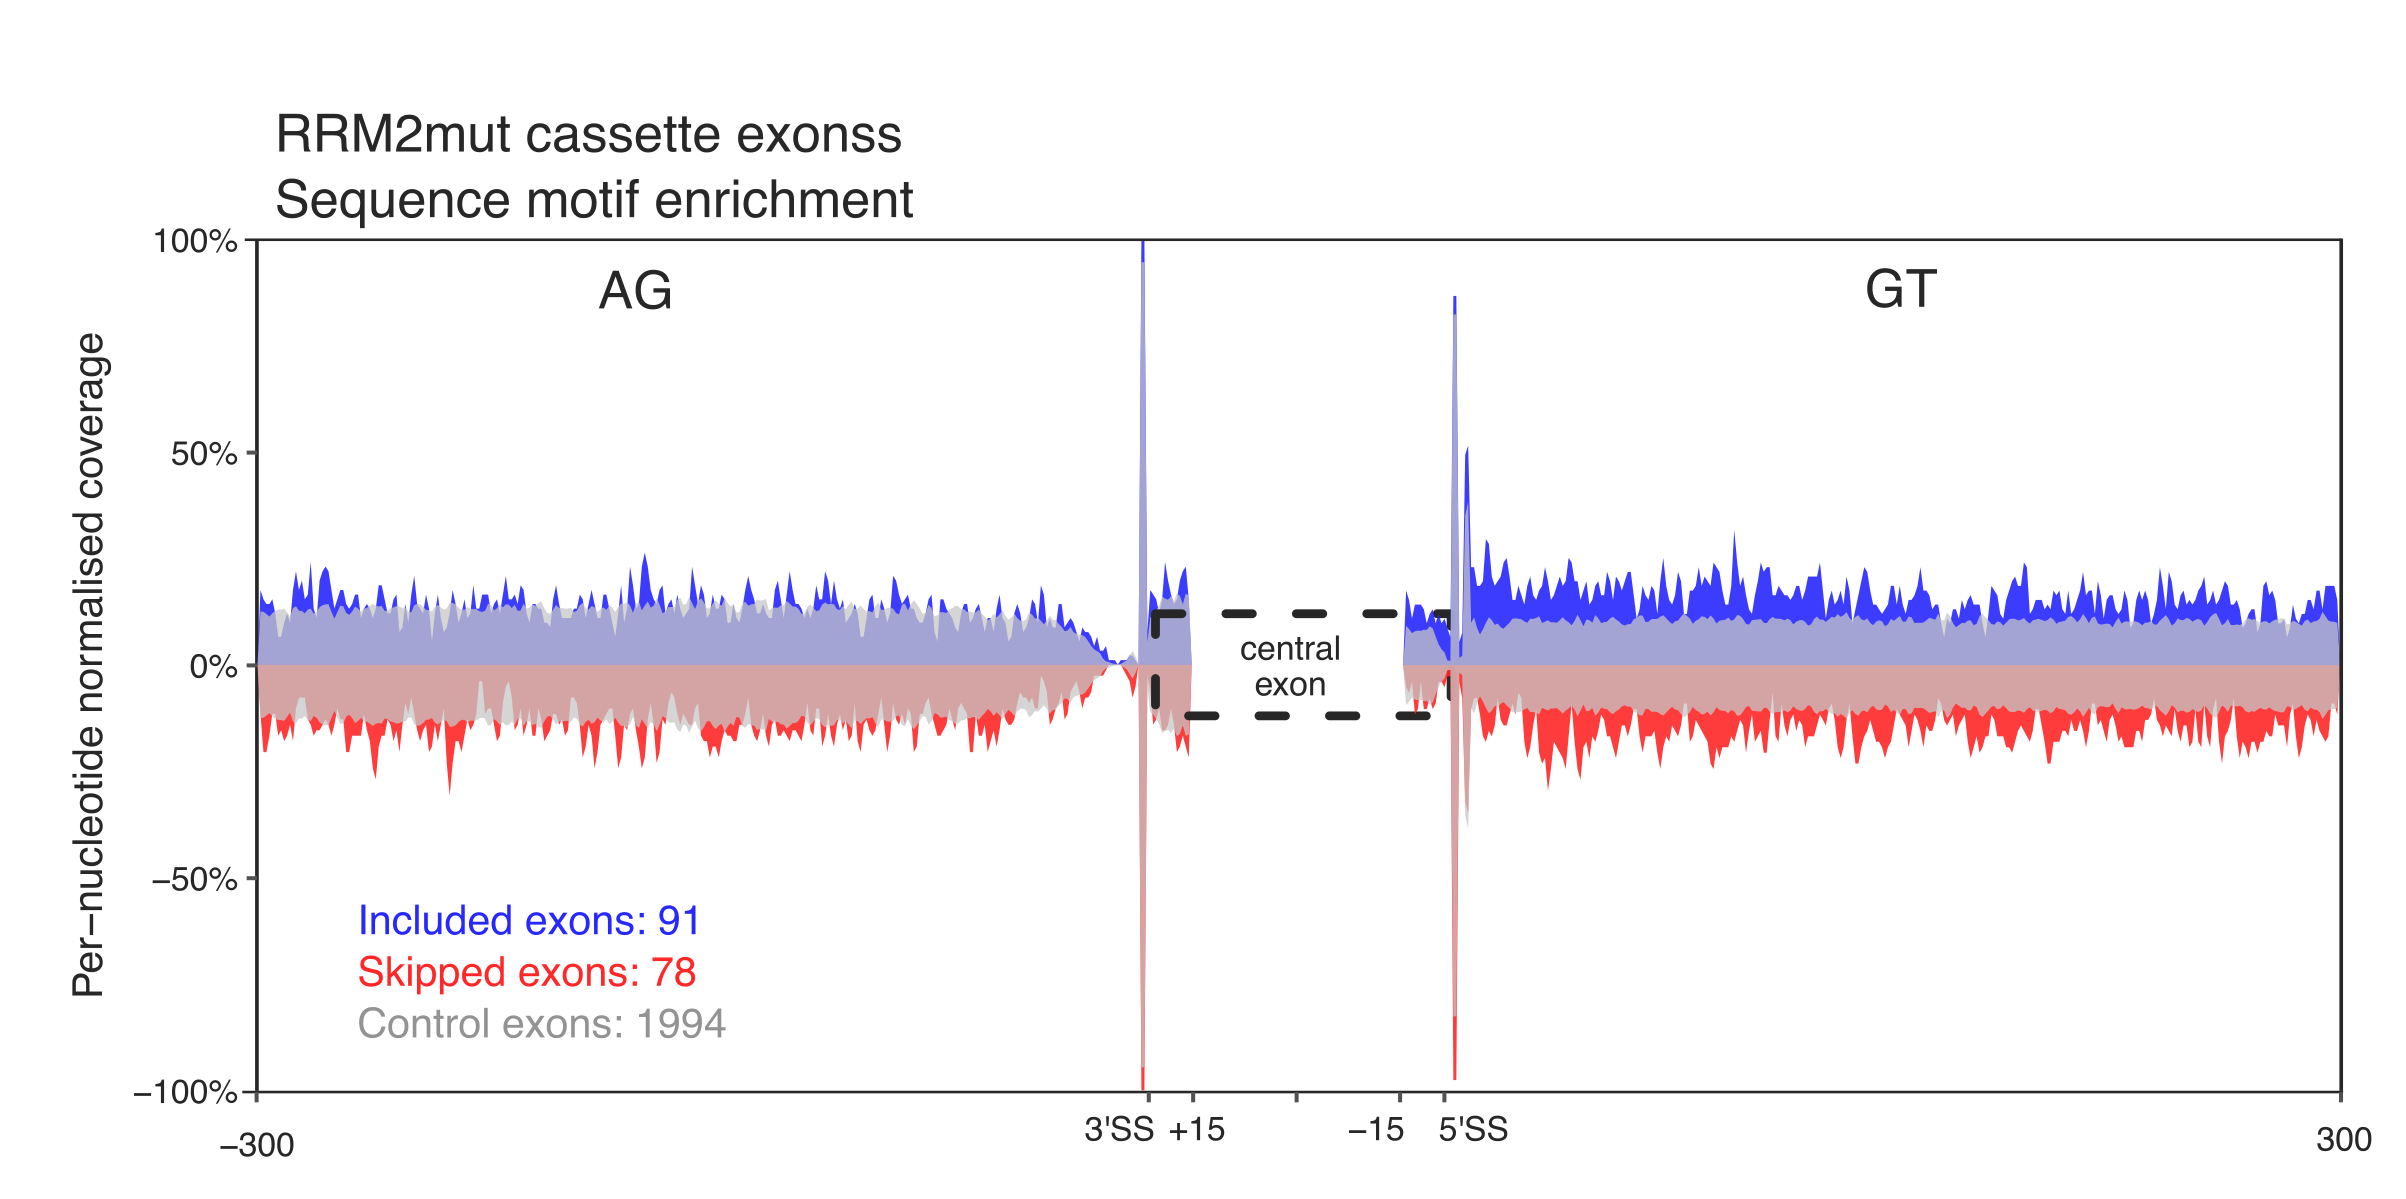
\includegraphics[width=14cm]{Figures/05_tdp_mice/RNAmap_motif_AG_GT_RRM2mut.png}
	\caption{\textbf{RNA maps of AG and GT dinucleotides are invariant at the 5' and 3' splice sites}}
	RNAmaps constructed from differentially included (blue) and skipped (red) cassette exons from RRM2mut.
	
	\label{fig:RNAmap_splicing}
\end{figure}


% Skiptic permutation

\begin{table}[!htbp] \centering 
	
	\footnotesize
	\caption{Results of permuting sample order and repeating splicing analysis. Exons refers to the number of differentially spliced exons found at FDR 5\%, cryptics are those that satisfy the cryptic exon critera and skiptics are those that satisfy the skiptic exon criteria (see chapter). Groups in bold are the correct sample ordering. Note that definitions of skiptic and cryptic depend on which condition is the reference, which accounts for the different numbers between the two correct orderings. } 
	\label{append:permutations} 
	\begin{tabular}{@{\extracolsep{5pt}} cccc} 
		\\[-1.8ex]\hline 
		\hline \\[-1.8ex] 
		groups & exons & cryptic & skiptic \\ 
		\hline \\[-1.8ex] 
		\textbf{M323K\_WT\_1+M323K\_WT\_2+M323K\_WT\_3+M323K\_WT\_4} & 920 & 2 & 47 \\ 
		\textbf{M323K\_HOM\_1+M323K\_HOM\_2+M323K\_HOM\_3+M323K\_HOM\_4} & 920 & 4 & 9 \\ 
		M323K\_HOM\_2+M323K\_HOM\_3+M323K\_HOM\_4+M323K\_WT\_3 & 38 & 0 & 0 \\ 
		M323K\_HOM\_1+M323K\_WT\_1+M323K\_WT\_2+M323K\_WT\_4 & 38 & 0 & 0 \\ 
		M323K\_HOM\_1+M323K\_HOM\_2+M323K\_HOM\_4+M323K\_WT\_4 & 25 & 0 & 1 \\ 
		M323K\_HOM\_3+M323K\_WT\_1+M323K\_WT\_2+M323K\_WT\_3 & 25 & 0 & 0 \\ 
		M323K\_HOM\_1+M323K\_HOM\_3+M323K\_HOM\_4+M323K\_WT\_4 & 25 & 0 & 2 \\ 
		M323K\_HOM\_2+M323K\_WT\_1+M323K\_WT\_2+M323K\_WT\_3 & 25 & 1 & 0 \\ 
		M323K\_HOM\_1+M323K\_HOM\_2+M323K\_HOM\_3+M323K\_WT\_1 & 24 & 0 & 0 \\ 
		M323K\_HOM\_4+M323K\_WT\_2+M323K\_WT\_3+M323K\_WT\_4 & 24 & 0 & 0 \\ 
		M323K\_HOM\_2+M323K\_WT\_1+M323K\_WT\_2+M323K\_WT\_4 & 24 & 1 & 0 \\ 
		M323K\_HOM\_1+M323K\_HOM\_3+M323K\_HOM\_4+M323K\_WT\_3 & 24 & 0 & 0 \\ 
		M323K\_HOM\_1+M323K\_WT\_1+M323K\_WT\_2+M323K\_WT\_3 & 19 & 0 & 0 \\ 
		M323K\_HOM\_2+M323K\_HOM\_3+M323K\_HOM\_4+M323K\_WT\_4 & 19 & 1 & 0 \\ 
		M323K\_HOM\_1+M323K\_HOM\_2+M323K\_HOM\_4+M323K\_WT\_2 & 17 & 0 & 0 \\ 
		M323K\_HOM\_1+M323K\_HOM\_2+M323K\_HOM\_3+M323K\_WT\_3 & 15 & 0 & 0 \\ 
		M323K\_HOM\_4+M323K\_WT\_1+M323K\_WT\_2+M323K\_WT\_4 & 15 & 0 & 0 \\ 
		M323K\_HOM\_2+M323K\_HOM\_3+M323K\_HOM\_4+M323K\_WT\_1 & 12 & 0 & 0 \\ 
		M323K\_HOM\_1+M323K\_HOM\_2+M323K\_HOM\_3+M323K\_WT\_4 & 7 & 0 & 0 \\ 
		M323K\_HOM\_1+M323K\_HOM\_3+M323K\_HOM\_4+M323K\_WT\_2 & 7 & 0 & 0 \\ 
		M323K\_HOM\_4+M323K\_WT\_1+M323K\_WT\_2+M323K\_WT\_3 & 7 & 0 & 0 \\ 
		M323K\_HOM\_3+M323K\_WT\_2+M323K\_WT\_3+M323K\_WT\_4 & 7 & 0 & 0 \\ 
		M323K\_HOM\_1+M323K\_HOM\_3+M323K\_HOM\_4+M323K\_WT\_1 & 5 & 0 & 0 \\ 
		M323K\_HOM\_2+M323K\_WT\_2+M323K\_WT\_3+M323K\_WT\_4 & 5 & 0 & 0 \\ 
		M323K\_HOM\_3+M323K\_WT\_1+M323K\_WT\_2+M323K\_WT\_4 & 2 & 0 & 0 \\ 
		M323K\_HOM\_1+M323K\_HOM\_2+M323K\_HOM\_3+M323K\_WT\_2 & 1 & 0 & 0 \\ 
		M323K\_HOM\_4+M323K\_WT\_1+M323K\_WT\_3+M323K\_WT\_4 & 1 & 0 & 0 \\ 
		M323K\_HOM\_3+M323K\_HOM\_4+M323K\_WT\_3+M323K\_WT\_4 & 51 & 0 & 0 \\ 
		M323K\_HOM\_1+M323K\_HOM\_4+M323K\_WT\_1+M323K\_WT\_4 & 11 & 0 & 0 \\ 
		M323K\_HOM\_2+M323K\_HOM\_3+M323K\_WT\_2+M323K\_WT\_3 & 11 & 0 & 0 \\ 
		M323K\_HOM\_1+M323K\_HOM\_2+M323K\_WT\_1+M323K\_WT\_3 & 11 & 1 & 0 \\ 
		M323K\_HOM\_3+M323K\_HOM\_4+M323K\_WT\_2+M323K\_WT\_4 & 11 & 0 & 0 \\ 
		M323K\_HOM\_2+M323K\_HOM\_4+M323K\_WT\_3+M323K\_WT\_4 & 11 & 0 & 0 \\ 
		M323K\_HOM\_2+M323K\_HOM\_3+M323K\_WT\_1+M323K\_WT\_3 & 9 & 0 & 0 \\ 
		M323K\_HOM\_1+M323K\_HOM\_4+M323K\_WT\_2+M323K\_WT\_4 & 9 & 0 & 0 \\ 
		M323K\_HOM\_1+M323K\_HOM\_2+M323K\_WT\_3+M323K\_WT\_4 & 9 & 0 & 0 \\ 
		M323K\_HOM\_3+M323K\_HOM\_4+M323K\_WT\_1+M323K\_WT\_2 & 9 & 0 & 0 \\ 
		M323K\_HOM\_2+M323K\_HOM\_3+M323K\_WT\_1+M323K\_WT\_4 & 9 & 0 & 0 \\ 
		M323K\_HOM\_2+M323K\_HOM\_3+M323K\_WT\_3+M323K\_WT\_4 & 7 & 0 & 0 \\ 
		M323K\_HOM\_1+M323K\_HOM\_4+M323K\_WT\_1+M323K\_WT\_2 & 7 & 0 & 0 \\ 
		M323K\_HOM\_3+M323K\_HOM\_4+M323K\_WT\_2+M323K\_WT\_3 & 6 & 0 & 0 \\ 
		M323K\_HOM\_1+M323K\_HOM\_2+M323K\_WT\_1+M323K\_WT\_4 & 6 & 0 & 0 \\ 
		M323K\_HOM\_2+M323K\_HOM\_3+M323K\_WT\_1+M323K\_WT\_2 & 4 & 0 & 0 \\ 
		M323K\_HOM\_1+M323K\_HOM\_4+M323K\_WT\_3+M323K\_WT\_4 & 4 & 0 & 0 \\ 
		M323K\_HOM\_1+M323K\_HOM\_2+M323K\_WT\_2+M323K\_WT\_4 & 4 & 0 & 1 \\ 
		M323K\_HOM\_2+M323K\_HOM\_3+M323K\_WT\_2+M323K\_WT\_4 & 3 & 0 & 0 \\ 
		M323K\_HOM\_3+M323K\_HOM\_4+M323K\_WT\_1+M323K\_WT\_4 & 21 & 0 & 1 \\ 
		M323K\_HOM\_2+M323K\_HOM\_4+M323K\_WT\_2+M323K\_WT\_4 & 18 & 0 & 0 \\ 
		M323K\_HOM\_1+M323K\_HOM\_3+M323K\_WT\_3+M323K\_WT\_4 & 16 & 0 & 0 \\ 
		M323K\_HOM\_2+M323K\_HOM\_4+M323K\_WT\_1+M323K\_WT\_2 & 16 & 0 & 0 \\ 
		M323K\_HOM\_1+M323K\_HOM\_3+M323K\_WT\_2+M323K\_WT\_4 & 14 & 0 & 1 \\ 
		M323K\_HOM\_2+M323K\_HOM\_4+M323K\_WT\_1+M323K\_WT\_4 & 2 & 0 & 0 \\ 
		\hline \\[-1.8ex] 
	\end{tabular} 
\end{table} 

% fibroblast sample info
\begin{table}[!htbp] \centering 
	\caption{Information on human fibroblast lines used. B,	bulbar;	UL, upper limb;	LL,	lower limb} 
	\label{append:fibros} 
	\begin{tabular}{@{\extracolsep{5pt}} ccccccc} 
		\\[-1.8ex]\hline 
		\hline \\[-1.8ex] 
		Fibroblast line & Mutation & Diagnosis & Age at onset & Site of onset & Gender & Age at biopsy \\ 
		\hline \\[-1.8ex] 
		TARDBP 1 & G298S & ALS & 62 & LL & M & 64 \\ 
		TARDBP 2 & A382T & ALS & 59 & UL & F & 62 \\ 
		TARDBP 3 & A382T & ALS & 25 & LL & F & 31 \\ 
		TARDBP 4 & A382T & ALS & 67 & B & M & 69 \\ 
		CTRL 1 & . & Healthy & . & . & F & 67 \\ 
		CTRL 2 & . & Healthy & . & . & M & 64 \\ 
		CTRL 3 & . & Healthy & . & . & M & 67 \\ 
		CTRL 4 & . & Healthy & . & . & F & 69 \\ 
		\hline \\[-1.8ex] 
	\end{tabular} 
\end{table} 


% skiptics list
\begin{table}[!htbp] \centering 
	\caption{List of skiptic exons found in LCDmut adult brain} 
	\label{append:skiptics} 
	\footnotesize
\begin{tabular}{@{\extracolsep{5pt}} ccccccccc} 
	
	\\[-1.8ex]\hline 
	\hline \\[-1.8ex] 
	chr & start & end & Gene & PSI\textsubscript{WT} & PSI\textsubscript{LCDmut} & $\Delta$PSI & fold change & \textit{q} \\ 
	\hline \\[-1.8ex] 
	chr2 & 144502918 &144503031 & \textit{Dzank1} & 0.9795 & 0.8160 & $$-$0.164$ & 8.9942 & 1.57E$-45$ \\ 
	chr7 & 56157784 & 56163742 & \textit{Herc2} & 0.9983 & 0.7828 & $$-$0.216$ & 128.6068 & 4.71E$-42$\\ 
	chr5 & 29597184 & 29600641 & \textit{Ube3c} & 0.9894 & 0.7449 & $$-$0.244$ & 24.1694 & 1.62E$-40$\\ 
	chr10 & 78284350 & 78287847 & \textit{Agpat3} & 0.9964 & 0.9011 & $$-$0.095$ & 27.1469 & 1.73E$-32$ \\ 
	chr5 & 36947237 & 36952351 & \textit{Ppp2r2c} & 0.9993 & 0.9359 & $$-$0.063$ & 94.4229 & 1.71E$-26$\\ 
	chr1 & 118304691  &118304770& \textit{Tsn} & 0.9978 & 0.9012 & $$-$0.096$ & 44.3227 & 7.36E$-23$ \\ 
	chr6 & 113492124  & 113492258 & \textit{Creld1} & 1.0000 & 0.8747 & $$-$0.125$ & \textgreater 150 & 1.05E$-22$ \\ 
	chr12 & 50365712 & 50383400 & \textit{Prkd1} & 0.9804 & 0.4517 & $$-$0.529$ & 28.0231 & 4.99E$-18$\\ 
	chr4 & 19618357 & 19621928 & \textit{Wwp1} & 0.9984 & 0.9111 & $$-$0.087$ & 56.7242 & 2.13E$-17$ \\ 
	chr4 & 58817550 & 58820128 & \textit{AI314180} & 0.9981 & 0.9037 & $$-$0.094$ & 51.0528 & 1.49E$-16$\\ 
	chr19 & 38265097 & 38283970 & \textit{Lgi1} & 0.9847 & 0.8165 & $$-$0.168$ & 11.9947 & 1.09E$-14$\\ 
	chr11 & 101317623  &101317727 & \textit{Psme3} & 0.9632 & 0.8737 & $$-$0.090$ & 3.4328 & 2.61E$-14$\\ 
	chr7 & 56184707 & 56185835 & \textit{Herc2} & 0.9881 & 0.8836 & $$-$0.104$ & 9.8083 & 1.25E$-13$\\ 
	chr5 & 108642696  & 108642779& \textit{Tmem175} & 0.9514 & 0.7273 & $$-$0.224$ & 5.6106 & 6.73E$-12$\\ 
	chr11 & 45852192 & 45884332 & \textit{Clint1} & 0.9962 & 0.8842 & $$-$0.112$ & 30.5766 & 1.85E$-10$ \\ 
	chr10 & 7710647 & 7712501 & \textit{Lats1} & 0.9959 & 0.9221 & $$-$0.074$ & 19.0151 & 5.18E$-9$\\ 
	chr11 & 97242047 & 97244428 & \textit{Npepps} & 0.9954 & 0.9425 & $$-$0.053$ & 12.6145 & 5.99E$-9$\\ 
	chr11 & 100440040 & 100440086 & \textit{Nt5c3b} & 0.9709 & 0.8464 & $$-$0.125$ & 5.2820 & 1.21E$-7$\\ 
	chr17 & 22428565 & 22446797 & \textit{Zfp946} & 0.9530 & 0.6858 & $$-$0.267$ & 6.6817 & 5.79E$-7$ \\ 
	chr2 & 130713397  & 130713503& \textit{4930402H24Rik} & 0.9908 & 0.9386 & $$-$0.052$ & 6.6376 & 7.23E$-7$ \\ 
	chr13 & 13638376 & 13641067 & \textit{Lyst} & 0.9909 & 0.8287 & $$-$0.162$ & 18.8410 & 8.97E$-7$\\ 
	chr6 & 30439865 & 30444427 & \textit{Klhdc10} & 0.9721 & 0.8957 & $$-$0.076$ & 3.7346 & 1.97E$-6$\\ 
	chr19 & 40340146 & 40344356 & \textit{Sorbs1} & 0.9877 & 0.8305 & $$-$0.157$ & 13.7569 & 2.29E$-6$\\ 
	chr5 & 8143132 & 8145553 & \textit{Adam22} & 0.9881 & 0.8977 & $$-$0.090$ & 8.5959 & 4.96E$-6$ \\ 
	chr14 & 18630431 & 18888266 & \textit{Ube2e2} & 0.9542 & 0.8915 & $$-$0.063$ & 2.3700 & 8.43E$-6$\\ 
	chr7 & 126153199 & 26153279 & \textit{Xpo6} & 0.9657 & 0.8754 & $$-$0.090$ & 3.6328 & 2.37E$-5$ \\ 
	chr8 &  105194475 & 105194591 & \textit{Cbfb} & 0.9736 & 0.8752 & $$-$0.098$ & 4.7209 & 4.06E$-5$ \\ 
	chr6 & 8216470 & 8224555 & \textit{Mios} & 0.9674 & 0.9026 & $$-$0.065$ & 2.9852 & 0.000146 \\ 
	chr5 & 9131308 & 9136066 & \textit{Dmtf1} & 0.9683 & 0.8230 & $$-$0.145$ & 5.5848 & 0.00015 \\ 
	chr16 & 17845135 & 17856752 & \textit{Dgcr2} & 0.9879 & 0.9334 & $$-$0.054$ & 5.4902 & 0.000182 \\ 
	chr16 & 94408716 & 94410833 & \textit{Ttc3} & 0.9925 & 0.8888 & $$-$0.104$ & 14.8993 & 0.000244 \\ 
	chr4 & 59592318 & 59594396 & \textit{Hsdl2} & 0.9801 & 0.9262 & $$-$0.054$ & 3.7039 & 0.000247 \\ 
	chr2 & 69741693 & 69746028 & \textit{Ppig} & 0.9725 & 0.9024 & $$-$0.070$ & 3.5489 & 0.00025 \\ 
	chr7 & 141526432  & 141526493 & \textit{Chid1} & 0.9876 & 0.9272 & $$-$0.060$ & 5.8899 & 0.000367 \\ 
	chr11 & 79242156 & 79244463 & \textit{Wsb1} & 0.9588 & 0.8991 & $$-$0.060$ & 2.4516 & 0.000532 \\ 
	chr1 & 119706155  & 119706313 & \textit{Ptpn4} & 0.9793 & 0.8764 & $$-$0.103$ & 5.9574 & 0.000597 \\ 
	chr10 & 83737933 & 83758134 & \textit{1500009L16Rik} & 0.9938 & 0.8995 & $$-$0.094$ & 16.2830 & 0.000837 \\ 
	chr8 & 75051657 & 75052150 & \textit{Tom1} & 0.9947 & 0.9301 & $$-$0.065$ & 13.2732 & 0.000883 \\ 
	chr11 & 58848702 & 58856061 & \textit{Gm12258} & 1.0000 & 0.8671 & $$-$0.133$ & \textgreater 150 & 0.000917 \\ 
	chr9 & 55858525 & 55859748 & \textit{Scaper} & 1.0000 & 0.8226 & $$-$0.177$ & \textgreater 150 & 0.001059 \\ 
	chr17 & 34905456 & 34905910 & \textit{Ehmt2} & 0.9718 & 0.8790 & $$-$0.093$ & 4.2930 & 0.001613 \\ 
	chr14 & 56957103 & 56959715 & \textit{Zmym2} & 0.9958 & 0.9412 & $$-$0.055$ & 14.0286 & 0.001684 \\ 
	chr5 & 110396045 & 110396074& \textit{Fbrsl1} & 0.9800 & 0.7715 & $$-$0.208$ & 11.4248 & 0.002646 \\ 
	chr5 & 3610288 & 3615075 & \textit{Pex1} & 1.0000 & 0.8614 & $$-$0.139$ & \textgreater 150 & 0.004794 \\ 
	chr9 & 54477528 & 54501351 & \textit{Dmxl2} & 0.9831 & 0.9073 & $$-$0.076$ & 5.4917 & 0.005274 \\ 
	chr17 & 75540191 & 75544748 & \textit{Fam98a} & 0.9778 & 0.8999 & $$-$0.078$ & 4.5140 & 0.0057 \\ 
	chr11 & 96773222 & 96776968 & \textit{Snx11} & 0.9873 & 0.9256 & $$-$0.062$ & 5.8572 & 0.008094 \\ 
	\hline \\[-1.8ex] 
	\end{tabular} 
	\end{table} 
	
\clearpage

\section{Appendices to \autoref{chapter:fus_meta} }

Scatter plots explainign the strict and relaxed overlaps

Imputing sex from chrY expression


\clearpage

\section{Publications}

I have attached 4 published papers in which I had a prominent role.


\subsection{Quantitative analysis of cryptic splicing associated with TDP-43 depletion}

I processed all the RNA-seq data. I designed and performed all analyses with advice and guidance from the other authors. I wrote the manuscript with advice and guidance from the other authors. I am the sole first author.

\subsection{Humanized mutant FUS drives progressive motor neuron degeneration without aggregation in \'FUSDelta14\' knockin mice}

I processed all the RNA-seq data. I designed and performed the differential expression and gene ontology analyses presented in Figure 4. I wrote the relevant methods section and assisted Dr Anny Devoy with intepretation of the data from my analyses.

\subsection{Mice with endogenous TDP-43 mutations exhibit gain of splicing function and characteristics of amyotrophic lateral sclerosis}

I processed all the RNA-seq data, assisted by Dr Kitty Lo. Dr Lo and I designed the splicing analyses together and I continued and finished the project after her departure. My work is included in Figures 2 and 5. I contributed to the writing of the manuscript and wrote all the relevant methods section. I received a joint first authorship credit.

\subsection{Annotation-free quanitification of RNA splicing with Leafcutter}

While on a short fellowship at Stanford University, USA, I was involved in the development of Leafcutter, a software package to run differential splicing analysis on RNA-seq data. I designed and created an interactive web-based application for users to visualise and explore the results of using the tool. A screenshot from the tool is used in Figure 1 of the paper. I am an active maintainer of the Leafcutter Github repository.

\clearpage

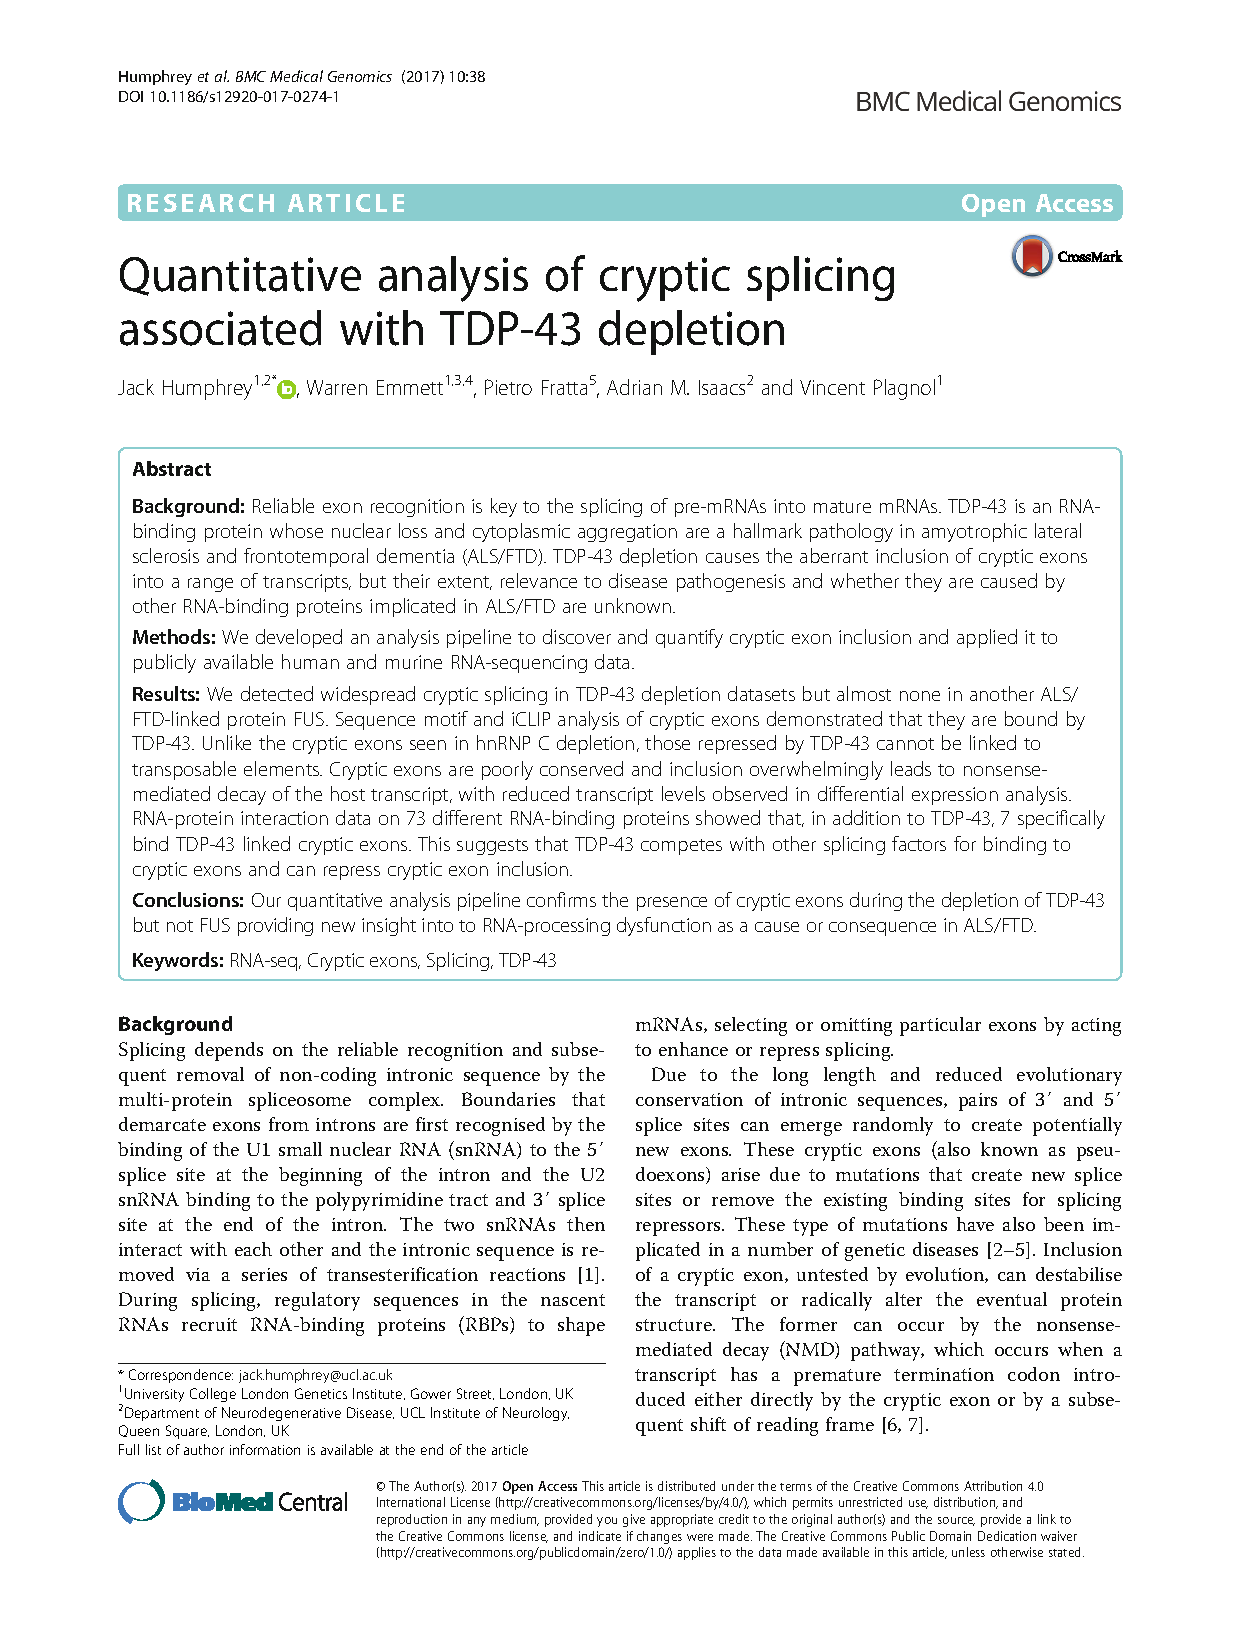
\includepdf[pages=-]{Appendices/Humphrey_Cryptic_Exons.pdf}
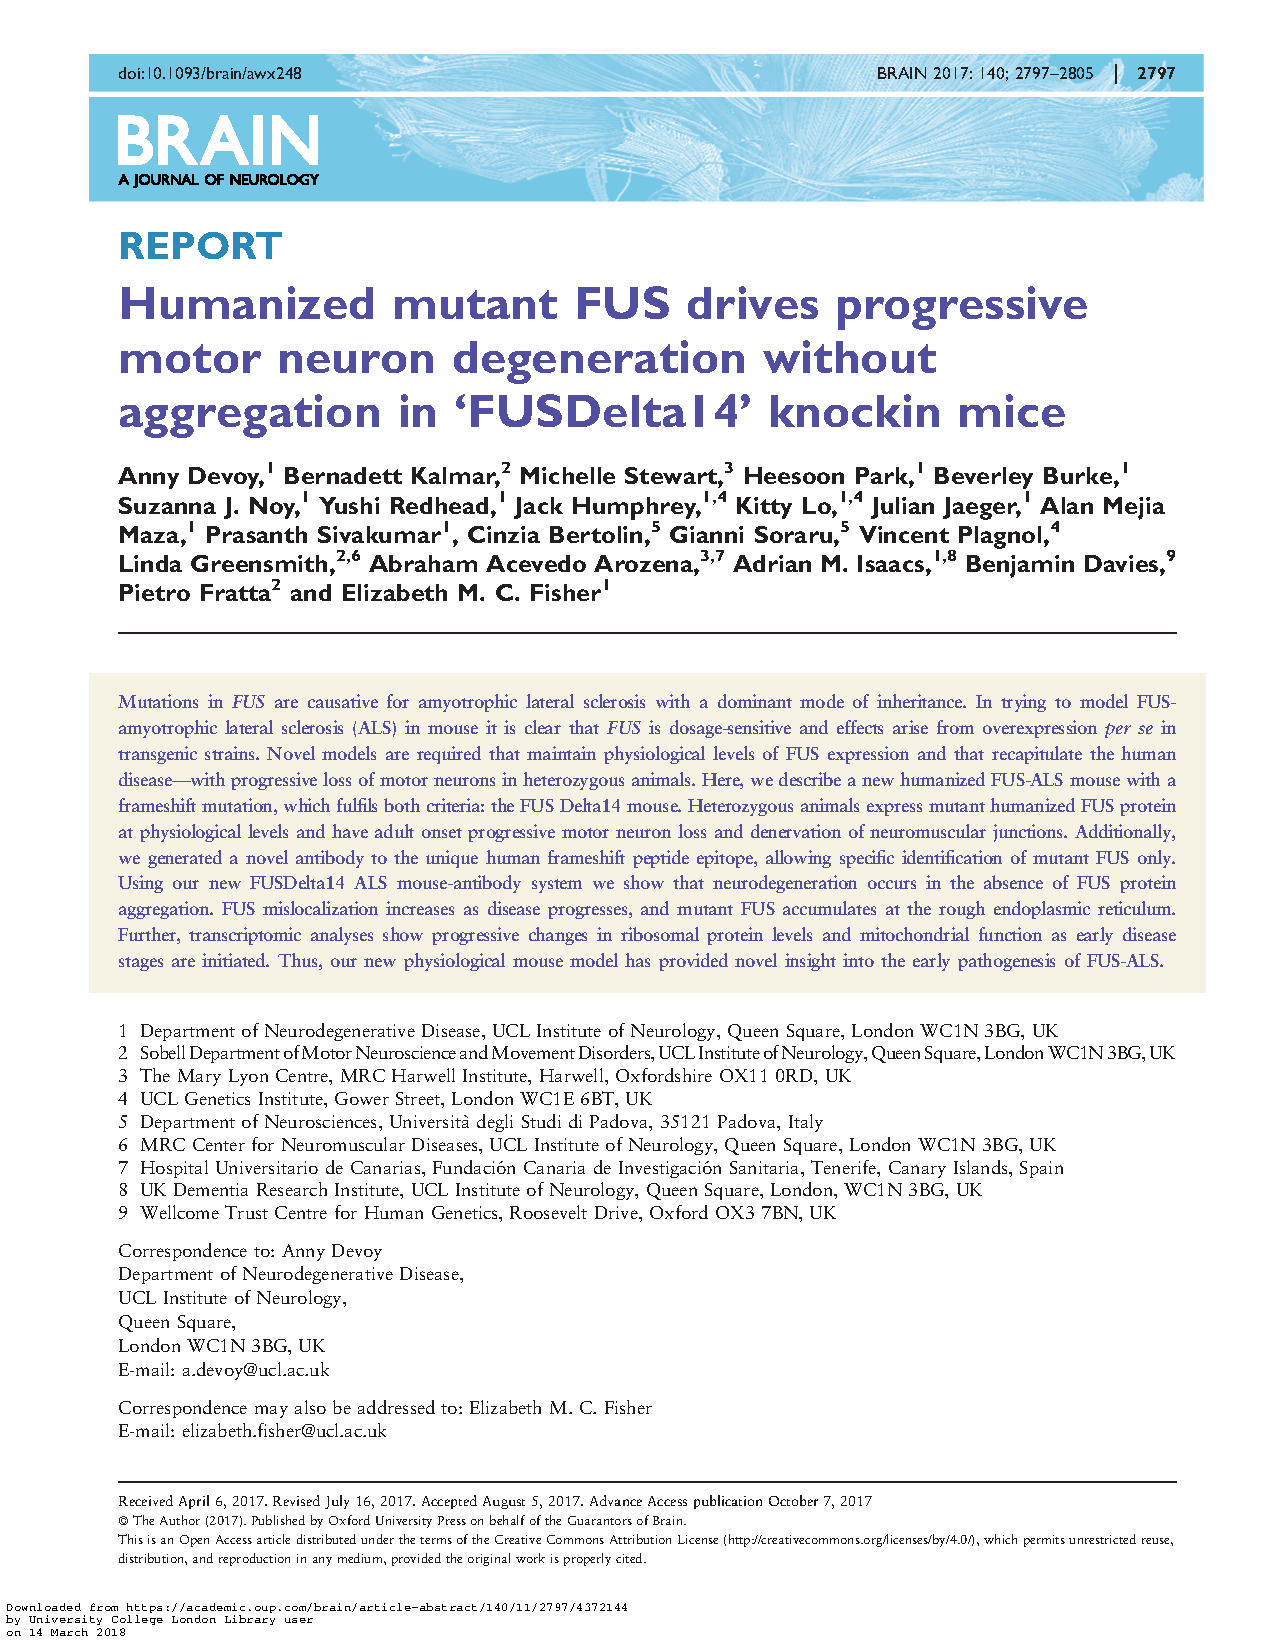
\includepdf[pages=-]{Appendices/Devoy_FUS_mouse.pdf}
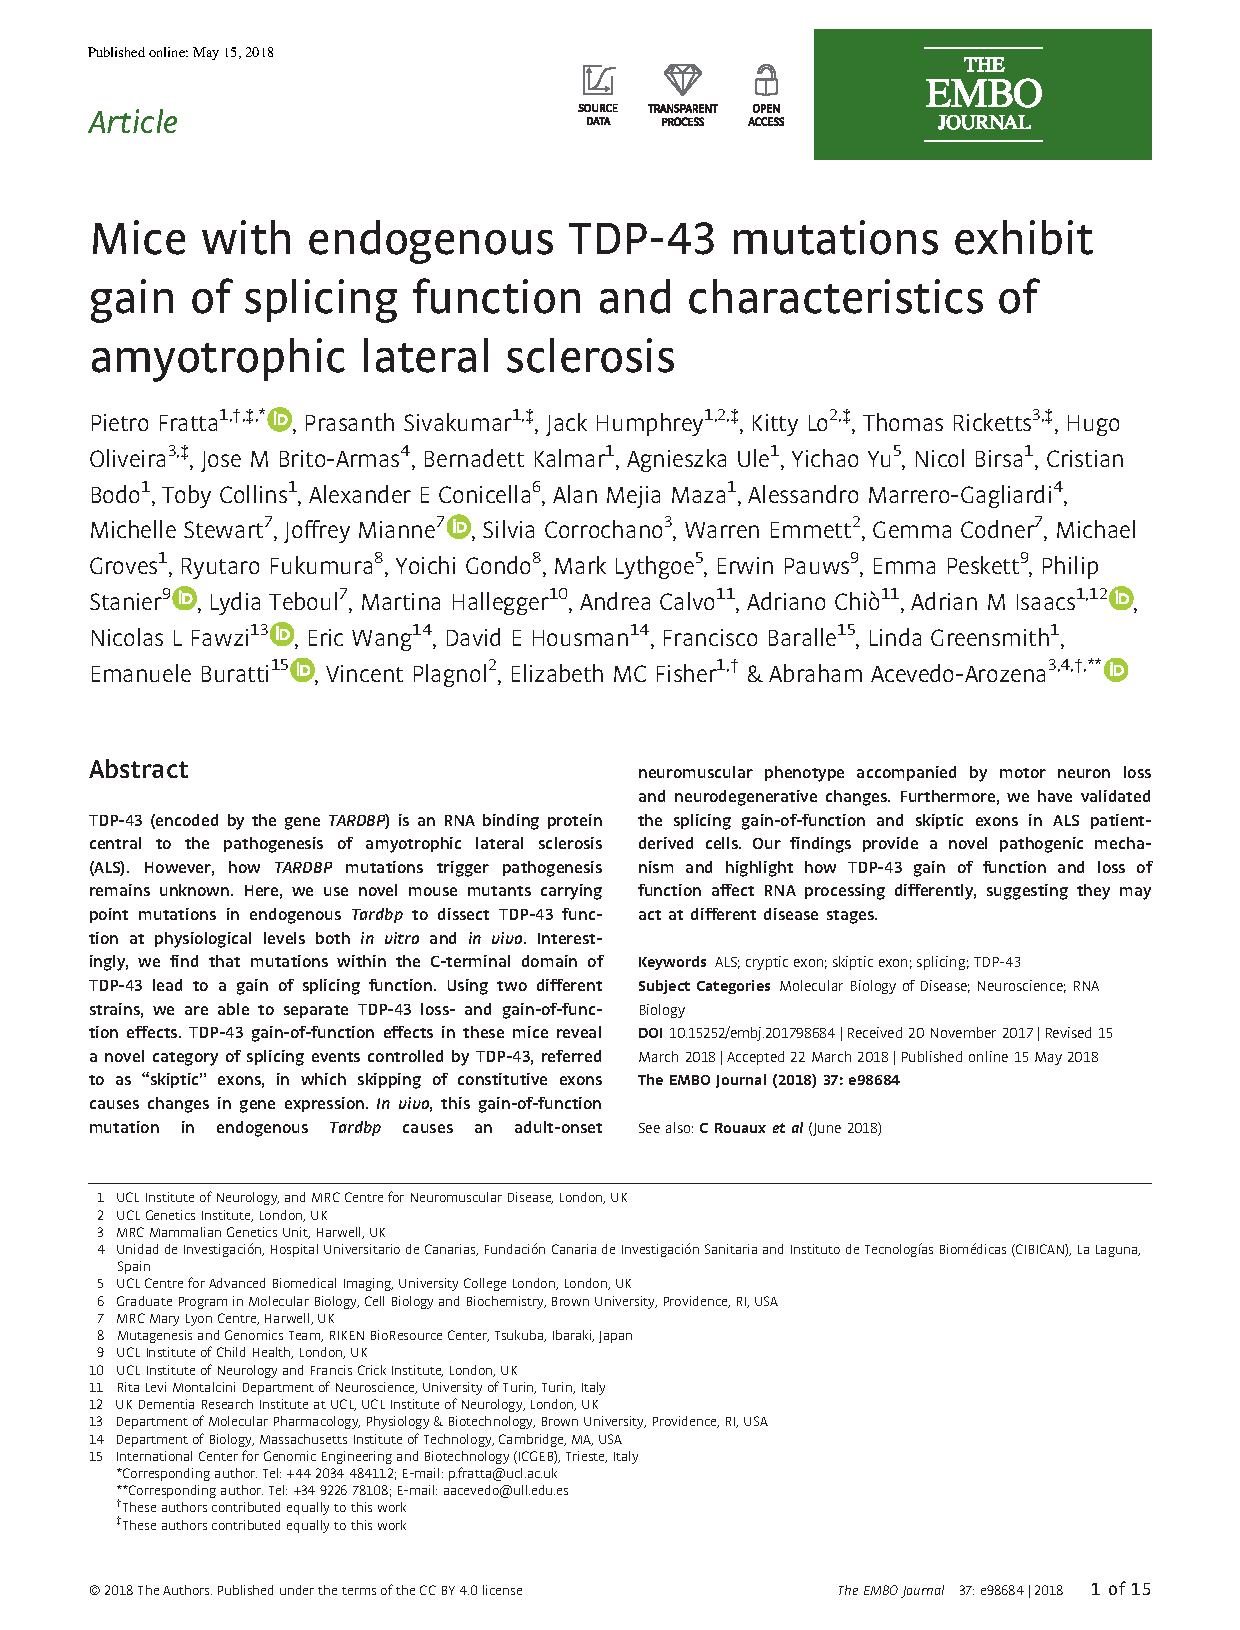
\includepdf[pages=-]{Appendices/Fratta_TDP_mice.pdf}
\includepdf[pages=1-9]{Appendices/Li_Leafcutter.pdf}

\end{appendices}